\documentclass[11pt]{article}

\usepackage{apacite}
\usepackage{amsmath}
\usepackage{amssymb,enumerate}
\usepackage{bibentry}
\usepackage{rotating}
\usepackage{caption}
\usepackage{array,multirow}

\usepackage[authoryear,round,longnamesfirst]{natbib}

\usepackage{enumitem}
\usepackage{setspace}
\linespread{1}
\usepackage{epsf,graphicx,psfrag}
\usepackage{lipsum}
\usepackage{framed}
\usepackage{graphicx}
\usepackage[export]{adjustbox}
\usepackage{geometry}
 \geometry{
 a4paper,
 total={210mm,297mm},
 left=25mm,
 right=25mm,
 top=25mm,
 bottom=25mm,
 }
\usepackage{pdflscape}
\usepackage{array}% http://ctan.org/pkg/array
\usepackage{color, colortbl}
\definecolor{Gray}{gray}{0.95}
\definecolor{LightGray}{gray}{0.85}
\definecolor{VLightGray}{gray}{0.75}
\definecolor{darkblue}{rgb}{0.0,0.0,.7}
\definecolor{shadecolor}{gray}{0.85}
\usepackage{color}
\usepackage{hyperref}
\hypersetup{colorlinks,breaklinks,linkcolor=darkblue,urlcolor=darkblue,anchorcolor=darkblue,citecolor=darkblue}
\usepackage{wrapfig}
\usepackage{CJKutf8}
\newcommand{\zh}[1]{\begin{CJK*}{UTF8}{gbsn}#1\end{CJK*}}

\usepackage{epigraph}
\setlength\epigraphwidth{16cm}
\setlength\epigraphrule{0pt}

\usepackage{etoolbox}
\usepackage{adjustbox}
\usepackage{xr}

\makeatletter
\patchcmd{\epigraph}{\@epitext{#1}}{\itshape\@epitext{#1}}{}{}
\makeatother

\interfootnotelinepenalty=10000
\usepackage{footnote}

\usepackage{float}

\title{The Logic of Informational Repression in China\thanks{\normalsize I would like to thank the National Science Foundation (Award \#1747397) and the Rackham Graduate School at the University of Michigan for their generous funding. I would also like to thank my research assistants, Qiwei Lin and Xinyue Xu for their help with text annotation and edits to survey questions. I would also like to thank Luciana Cingolani, Sasha de Vogel, Iza (Yue) Ding, Yilang Feng, King-Wa Fu, Yuequan Guo, Guo'er Liu, Ting Luo, Steven Moore, Jeffrey Javed, Aofei Lu, Walter Mebane, Jennifer Pan, Daniela Stockmann, Daniel Slater, Michael Thompson-Brusstar, Nicholas Valentino, and Nicole Wu for their helpful feedback.}\\ \large }

\author{Blake\ Miller\thanks{\normalsize{Assistant Professor, London School of Economics} (Email: \mbox{b.a.miller@lse.ac.uk})}}

\date{\today}

\newcommand{\cmmnt}[1]{}

\begin{document}
\maketitle

\begin{abstract}
\begin{normalsize}
In China, the state has fundamentally changed its information control strategies in response to the growing threat of virality on social media. In this paper, I outline the strategy of informational repression developed to combat this threat through cooperation between the state and internet communication technology companies (ICTs). Informational repression is a combination of covert information control and targeted repression. ICTs in China have increased linkages with state institutions, allowing surveillance and repression of carefully selected targets, and strategic cooptation of individuals with considerable influence on social media platforms. These dual strategies preserve the responsive and informational affordances of social media while mitigating the threat of social media as a conduit for instability. In this paper, I outline this strategy using evidence from government documents and process tracing of contention and cooperation between the state and ICTs. I then examine how this strategy works using a series of online experiments conducted in China. These experiments confirm that keeping information control covert is in both the government and private companies' best interests. Careful and covert information control, when paired with targeted repression, can mitigate the threat of virality while limiting backlash and chilling effects that can result from heavy-handed censorship. These findings demonstrate that the state and ICTs have converged upon a strategy of informational repression that maintains control over the internet while preserving a source of valuable information needed for responsiveness and control of threats to state control.
\end{normalsize}
\end{abstract}
\doublespacing

{\it Note: This is a very early draft. Many details of the process-tracing, experimental design, and treatment-blind survey response annotation have yet to be completed. Please do not share or distribute without permission.}

\section*{Introduction}

In China, the state has been experimenting with public opinion guidance in online social platforms for over two decades \citep{wei2015gongan,zou2015wangluo,xie2011zhongguo,xie2018zhongguo}. Over this period, the state has employed a mixed-strategy approach to information control, fitting into three main categories: content removal, content augmentation, and targeted repression. In this paper, I argue that the state and internet communication technology companies (ICTs) have converged upon a strategy of "informational repression" that targets individuals covertly, leaving as light a footprint as possible. This strategy is a significant departure from the widespread untargeted repression and censorship of the Mao- and early-Reform periods, and the categorical repression of the post-Tiananmen period (e.g., a categorical focus on well-organized, system-threatening collective action). Through a period of contestation with social media companies where state demand for content elimination was resisted by profit-minded ICTs, the state reluctantly gained an appreciation of softer, more targeted forms of repression and censorship. As \citep{han2018contesting} argues, impressions of pluralism and discourse competition in citizens' online interactions gives credence to state discourse without completely silencing competing discourse. In recent years, the state has learned to leverage the technological expertise of social media companies whose business model relies on effectively surveilling users' consumer preferences. Fine-grained surveillance of online behavior by technology companies is also useful for determining where the state should direct its repressive efforts. Leveraging digital surveillance to carefully target repression benefits the state in two ways. First, it limits the visibility of state interventions, giving individuals a perception of pluralism and discourse competition, and increasing their willingness to share their genuine opinions. Second, by carefully selecting citizens as targets of repression and censorship, the state avoids widespread backlash and chilling effects that often follow more brute-force, heavy-handed, or categorical censorship and repression.

In this paper, I focus on the first of these two benefits: how individuals respond to covert forms of repression in ways that benefit the state and ICTs alike. I trace the evolution of state involvement in—and contestation between the state and ICTs in China. I argue that through this contestation, a state strategy of informational repression has emerged. The strategy of informational repression combines digital surveillance and covert forms of repression to limit the visibility of state intervention, limiting backlash against the state and ICTs, while preserving the appearance of discourse competition online.

To explore how individuals respond to covert information control, I conduct online experiments with Chinese internet users. In these experiments, I present them with a fictional news aggregator, Now News, and direct them to test the platform before its future release. This platform is a fully functional news aggregator app that they can interact with as they would any news aggregator. A baseline version of the site will contain a mixture of favorable, neutral, and unfavorable comments about a proposed rideshare policy. To measure the effects of information control on perceptions of discourse competition, state support, and affinity for the fictional news aggregator, I randomly assign them to three different treatments which simulate three main categories of information control. An additive information control treatment includes additional favorable comments (astroturfing), a subtractive information control treatment removes all negative comments (content deletion), and a suppressive information control treatment informs them of content moderation of the platform. I also randomize the covertness of information control for each information control treatment. After instructing them to read the article and comments and explore the news aggregator platform, I ask them a series of post-treatment questions measuring their support for the rideshare policy, their experience on the fictional news aggregator platform, and their perception of discourse competition in the comments. I find that keeping information control covert is in both the government and private companies' best interests, as users in the covert treatment groups had appreciably more favorable views of both the state rideshare policy and the news aggregator site. Furthermore, those in covert treatment groups reported impressions of more discourse competition compared to those in overt treatment groups. These findings suggest that careful and covert information control, when paired with targeted repression, can mitigate the threat of virality while also limiting backlash and chilling effects that can result from heavy-handed censorship.

\section{The Logic of Informational Repression}

Recent scholarly work on repression has noted a decline in the visibility and overtness of violent repression \citep{fariss2014respect,fariss2019yes,guriev2019informational,hassan2022political} and an increase in softer, less visible forms of coercion---what \cite{davenport2005understanding} calls "covert repression." In China, this trend toward covert coercion has been noted in scholarly works on repression \citep{gallagher2021not,ong2018thugs} and censorship \citep{crete2016harmonize, ruan2021information, miller2018limits, miller2018delegated}. We know very little, however, about the state logic behind these changes in strategy, how they evolved, and how they influence citizens' compliance and attitudes toward the state.

In this paper, I argue that contention between ICTs and the Chinese state has led to the adoption of softer control methods. As ICTs mediate coercion in the online public sphere, conflicts often arise between the state and profit-minded ICTs who wish to limit censorship and repression, negatively impacting user experience. While early contestation was fierce, the state and social media companies reached an equilibrium. As evidenced in government documents, the state slowly realized that covert censorship, as implemented by profit-minded companies, was working in their favor. Keeping censorship and repression user-targeted, covert, and carried out by agents obscured state coercion from the view of average citizens. Partnerships and coercion between the state and ICTs allowed for careful curation of discourse through cooptation and repression of influential individuals rather than blanket bans on content which have backfired in the past. Encouraging those with considerable influence to operate within the bounds of acceptable discourse keeps state intervention in the online sphere hidden, thus benefitting the state's information-gathering efforts.

\subsection{Augmented Capacity through the Private Sector}

In 2011, the Chinese government began to experience a series of incidents that made the lack of effective control of explosively popular social media platforms surface. Starting with the Wenzhou train crash and culminating with the dramatic downfall of Chongqing Mayor Bo Xilai, the state found itself unable to control the narrative online. The urgency of the state's difficulty with social media became clear when Document Number Nine—which forcefully urged the Party to regain control of the ideological sphere online—was leaked.

After the experience of 2011 and 2012, the state made a strong push to augment the state's surveillance capacity by drawing on the technological expertise of the private sector. Hundreds of public opinion monitoring platforms emerged, with state-affiliated platforms from the People's Daily, the Global Times, and The Communist Youth League leading the charge. The state began to see social reach rather than categorical content bans as the way forward. A 2013 judicial interpretation reflected this insight and criminalized spreading rumors that were retweeted more than 500 times or viewed more than 5,000 times. \cite{miller2022improvising} and \cite{gallagher2021not} analyze the many government documents and manuals that were subsequently developed to help local governments build their online surveillance capacity. They found that a key focus of these documents was targeting online influence rather than content.

In 2014, Xi made efforts to consolidate control of the online sphere by reorganizing the regulatory institutions governing the internet, announcing the Cyberspace Administration of China. At this time, the government began focusing on artificial intelligence and big data as an economic objective but also as a critical pillar of social stability. AI and technological advancements in the private sector could help the state glean insights from the enormous social data generated online in China. In 2016, Xi called ICTs, "the Party's front line for public opinion work." Further, he focused his efforts on opinion leaders, saying, "we must strengthen education and guidance of online opinion leaders, we must encourage the good ones and restrain the bad ones, we cannot let things slide" \citep{creemers2017cyber}. According to a 2016 State Council document, in the first instance, surveillance and monitoring of public opinion were to be carried out by local governments \citep{statecouncil2016}. In response, a vast for-profit industry has emerged in China to identify threats, track public opinion ({\it yuqing}), and identify "emotional sentiment." State newspaper The Beijing News reports that nearly two million individuals work for hundreds of these public opinion monitoring platforms \citep{bjn2014}. These platforms purport to provide "public opinion early warning systems" that track errant content and identify who was the most instrumental in spreading that content. \cite{batke2020message} report on these for-profit companies in an analysis of thousands of procurement notices and corresponding documents, making clear the massive scope of this outsourced surveillance industry and the particular importance of opinion leaders as targets of state-outsourced surveillance. In 2020, the New York Times published a report on the enormous effort of these surveillance systems to control the narrative surrounding whistleblower Li Wenliang's death in the early days of the COVID-19 pandemic \citep{zhong2020no}.

A notable article in a Party journal by Ren Xianliang, the director of the Shaanxi provincial Propaganda Department, suggests that Weibo influencers have exceeded the reach of Party-dominated print media. He laments, "If we do not take this seriously, but take a laissez-faire attitude, a 'broken window' effect is bound to ensue [...] we must dare to boldly confront those powerful media, famous websites, famous bloggers and Weibo Big Vs in terms of management, warn those that should be warned, shut up those that should be shut up, and close those that should be closed" \citep{creemers2017cyber}. On a similar note local government cadre manuals on opinion guidance urge local governments to ``[Pay attention to] ‘Big V’ users who have many fans and followers... [because they] decide the development of online opinion events or the formation of topics of discussion.'' To preserve authenticity and credibility, the manual stresses that cadres, ``maintain the relative independence of opinion leaders [...] co-opt those with different points of view, deal with individuals on a case-by-case basis, support [those with the] ‘correct’ [opinion] and repress/co-opt [those with the] ‘wrong’ [opinion].''

To supplement active monitoring of influential "Big V" users, the Party has focused on developing its own army of influencers. A cadre manual on "responsive governance and opinion response on Weibo" suggests that it is important to ``institutionalize specially selected opinion leaders, discover, cultivate, and train opinion leaders, as well as encouraging leadership cadres to act as opinion leaders.'' Over the last several years, social influence of local governments has become a part of cadre evaluation, with metrics and rankings of local government bureaucracies published annually by the People’s Daily Online Public Opinion Monitoring Center. By co-opting those outside the Party and building influence within the Party, the state has made great strides to control counter-hegemonic spaces online and increase the discourse power of the state \citep{gallagher2019who}.

\subsection{Exerting Control over ICTs}

{\it [To be added, review of regulation of social media companies, Party organizations within social media companies, and government investment/threats of expropriation.]}

\subsection{Targeting Repression}

How a state targets repression can have serious downstream consequences for collection of actionable intelligence on political threats. Indiscriminate, wide-scale repression, censorship, or propaganda can interfere with information collection by creating chilling effects or backlash from those who experience repression. This dilemma has been widely noted in recent literature on information control in China. \cite{huang2018pathology} finds that "hard" propaganda—overt, heavy-handed propaganda—is less convincing than softer, more covert propaganda. Relatedly, \cite{han2018contesting} argues that the perception that the state less heavily moderates online spaces can lead users to believe that the Party's narrative is indeed the dominant narrative.

Further, the belief that the state does not heavily moderate the public sphere can prevent chilling effects that might adulterate the online public sphere, which serves as a reservoir of information on public opinion threats. \cite{gallagher2021not} find that the state is also careful about targeting censorship and repression to a particular subset of users with influence and social reach on the platform. This cautious targeting, I argue, has given the state in China a more credible read on public opinion in its surveillance of social media. 

Backlash and chilling effects can also be avoided by delegating censorship to non-government agents. In China, information control is carried out indirectly through directives to ICTs (cite my diss, cite the Esarey piece, cite Chris). It is thus unclear if information control or repression is being carried out by the state or an overzealous ICT platform. For example, when blanket censorship of LGBT content on Weibo resulted in an intense public backlash, the state blamed Sina's management and denied involvement in the censorship policy. Similarly, the state outsources violent repression to organized criminals and thugs to evict homeowners, enforce the one-child policy, and demobilize protesters and petitioners \citep{ong2018thugs}. As Ong argues, the state utilizes these tactics to "evade responsibility" and "augment the state's lack of capacity," going to great lengths to hide repression from view by carrying out their attacks late at night.

%Targets
%\citep{rozenas2020theory}
%\citep{feldstein2019artificial}
%\citep{xu2021repress}
%\citep{han2021scaling}
%\citep{sun2022delegated}
%\citep{xu2022information}
%\citep{bolsover2019chinese}

%Influencers
%\citep{su2019exploring}
%\citep{woolley2022digital}
%\citep{huang2018propaganda}
%\citep{neagli2021grassroots}

\subsection{Plausible Deniability}

In addition to the informational affordances of more covert political control tactics, limiting the scope of censorship to those with influence can prevent a costly backlash that can be counterproductive to the state's information control efforts. \cite{roberts2015experiencing,roberts2017censorship} has identified multiple instances where heavy-handed censorship has encouraged individuals to circumvent China's "Great Firewall" to seek out information that has been categorically hidden from view. Narrowing the scope of state targets of coercion and cooptation aids the state's political control efforts by limiting the potential for any fallout that may ensue because of repression.

\section{Overview and Typology of Information Control}\label{types_info_ctrl}

Information control is the systematic government manipulation of the visibility of information to the public. I suggest three main sub-types of information control based on how one can change the visibility of information: adding favorable information (using astroturfing, propaganda, etc.), subtracting unfavorable information (through deletion, shadow-banning\footnote{Shadow-banning is an information control tactic that is meant to prevent users from discovering that they have been censored. To users who have been shadow-banned, their post appears to be visible from the perspective of their user account (it might appear on their profile), while the post is invisible to all other users.}, etc.), or suppressing the expression of latent unfavorable information (by intimidating, threatening, or co-opting regime critics). In \hyperref[info_manip_dist]{Figure \ref*{info_manip_dist}}, I visualize these three subtypes of information control using a symmetric univariate distribution representing the probability that an individual receives information of a particular polarity (positive to negative). Positive values represent information favorable to the government, and negative values represent information unfavorable to the government. The government's goal in its information interventions is to make favorable information more visible and make unfavorable information less visible. Assuming that an unperturbed distribution of information is symmetric around a neutral viewpoint, \hyperref[info_manip_dist]{Figure \ref*{info_manip_dist}} depicts three ways the government could shift the mean opinion toward the same positive value $\mu^*$.

Though the average polarity of each of the three methods of information control visualized is identical, the variation in polarity across these three methods of information control differs significantly. The additive distribution, for example, has some probability mass at the negative tail, the suppressive distribution has slightly less, and the subtractive distribution does not have any.

Each intervention results in a distribution of information polarity with different levels of discourse competition. To the information consumer, the additive distribution would appear to have the most discourse competition, the suppressive distribution would have a small amount of discourse competition, and the subtractive distribution would have no discourse competition.

\begin{minipage}{\linewidth}
    \begin{center}
      \singlespacing
      \captionof{figure}{Three Main Information Control Tactics}
      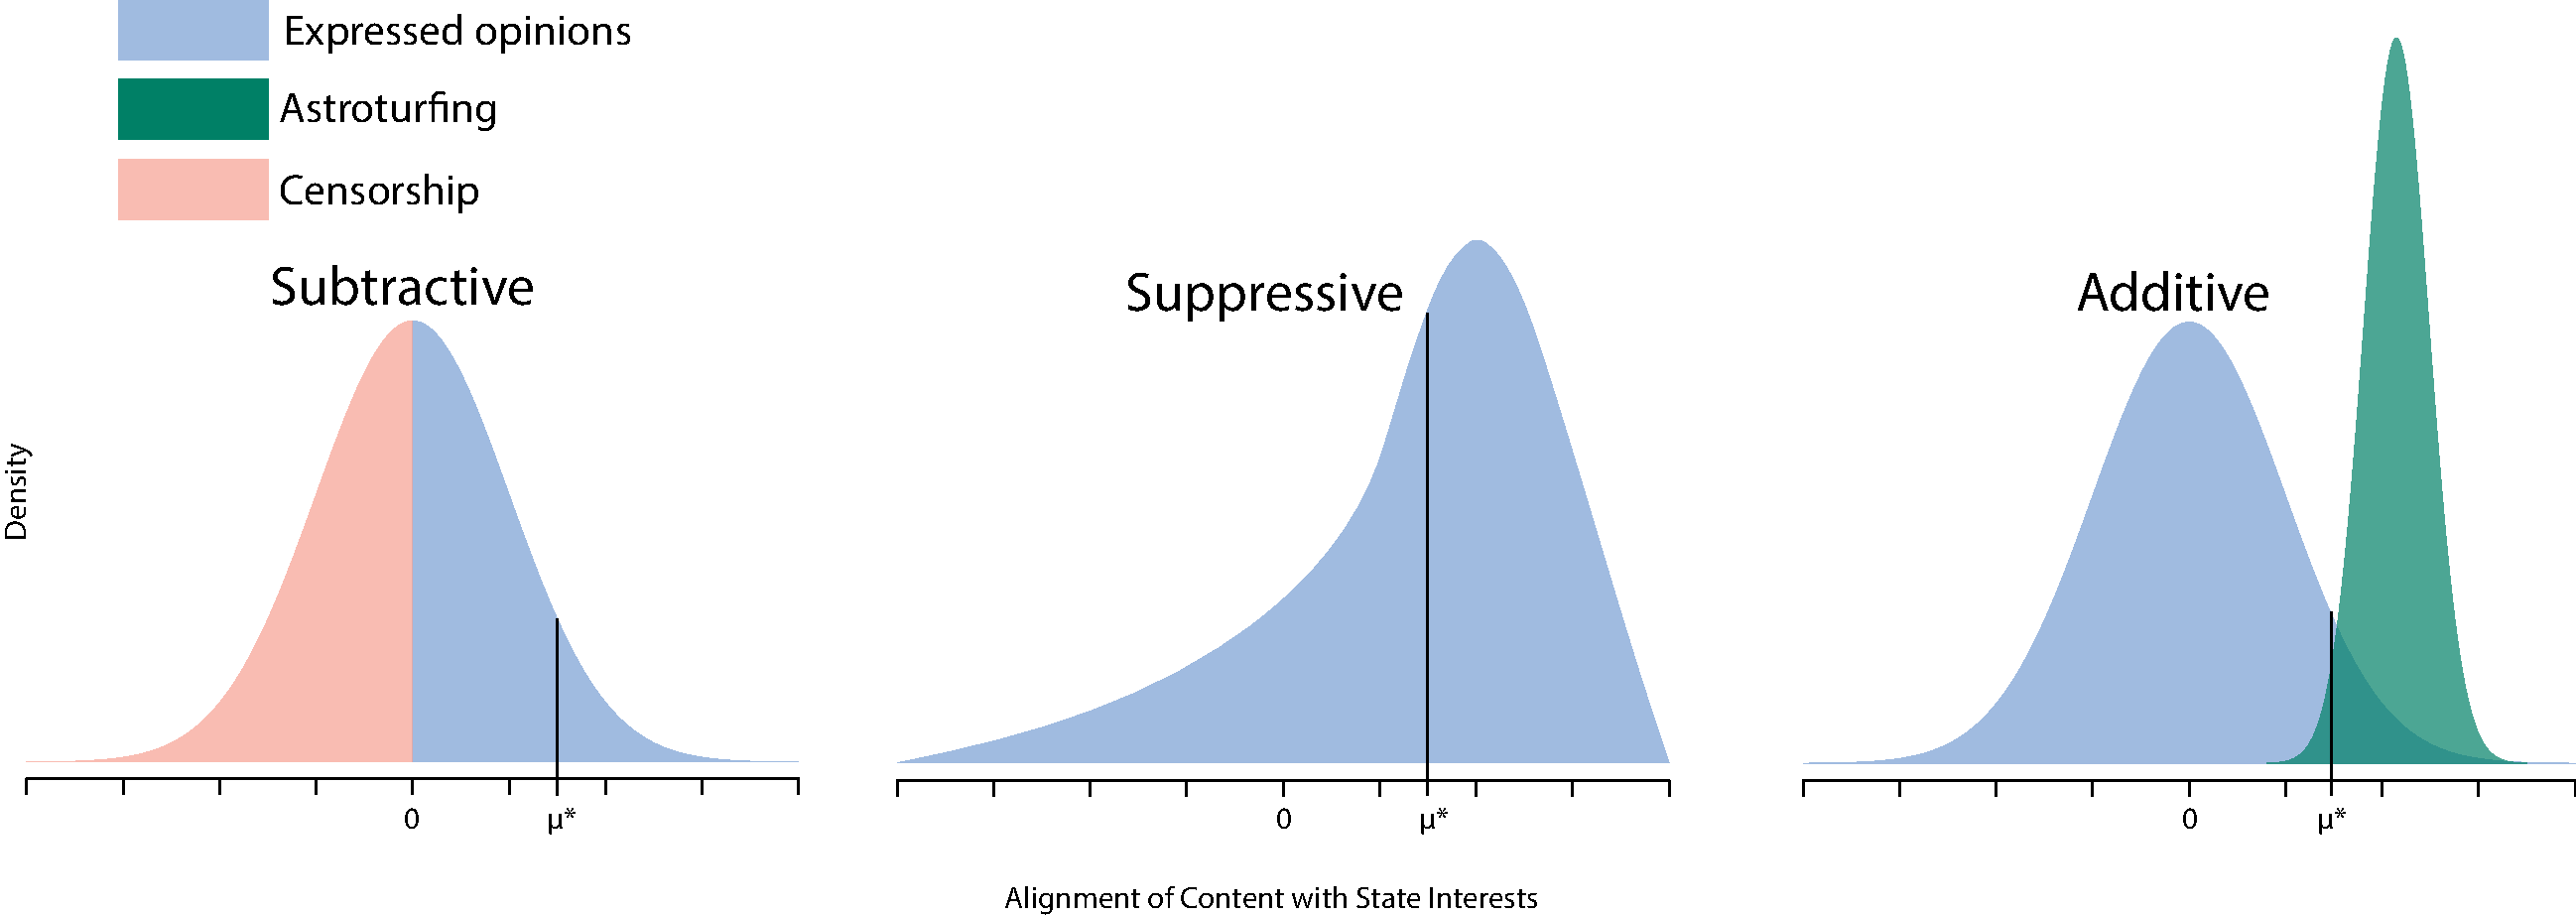
\includegraphics[width=\textwidth]{figures/info_manip_dist.pdf}\\
      \scriptsize{\it If the true density of opinions held by individuals in society is assumed to be symmetric around neutral viewpoint (zero), each of the three plots is an illustration of how each of three major information manipulation tactics can move the visible and expressed opinions toward the state's ideal, $\mu_{+}$.}\vspace{2em}
      \label{info_manip_dist}
    \end{center}
\end{minipage}

These three types of information control can also vary in their conspicuousness. In additive information manipulation, the state's identity as the information manipulator is sometimes present and sometimes obscured. In some circumstances, government bureaucrats participate in online discourse openly with the identity of a bureaucrat (i.e. their name and title are visible in their social media profile, they wear a uniform in their profile picture, or are posting from an official government account). In other circumstances, the bureaucrat will deliberately obscure her identity to appear like she is an ordinary citizen. Each type of information control in \hyperref[info_manip_dist]{Figure \ref*{info_manip_dist}} has overt and covert forms.

Of course, each of these tactics themselves differ in the degree to which the information manipulation is observed and the degree to which the identity of the information manipulator is identifiable. Subtractive information manipulation, for example, can only be overt or covert if the deletion of content is reported to the user, which in some cases it is. In most cases, comments are deleted without notice to the user. Suppressive and additive information control are more conspicuous in overt and covert forms than most subtractive information. Because suppressive information control seeks to dissuade individuals from posting anti-regime messages using carrots and sticks, the information control tactic is almost always observed. In additive information control, the information control tactic can be observed in the overt form if the resulting distribution of opinions is so skewed that it does not seem plausible to the user. In overt forms, the presence of opinions from state-affiliated individuals means this information control tactic is observed.

\section{Evidence from Government Policies Source Documents}

{\setstretch{1}
\epigraph{``Any dissemination of information involves an information selection process. During the process, there are a variety of `gatekeepers' such as content editors and webmasters who play a very important role in information selection and opinion guidance. These `gatekeepers' should not simply delete comments but focus on the art of guidance so as to persuade and move the masses.''\footnotemark\newline}{--- {\it Weibo Government Platforms and Responsiveness to Public Opinion} \citep[155]{zhang2014weibowenzheng}}}
\footnotetext{Original Chinese text: ``\zh{任何信息的传播都是信息选择的过程,期间充满了各种各样的“把关人”。网络“把关人”包括网站编辑,网管等,他们在信息选择,引导舆论方面至关重要。这些网络“把关人”在工作中,切记简单粗暴地删帖,注重运用动之以情,晓之以理的引导艺术,使网民产生理性和感情上的认同和共鸣。}''}

The Chinese public has grown accustomed to contestation and pluralism in the public sphere \citep{han2018contesting,lei2019contentious}. While Chinese citizens understand that the state regulates information through censorship and media controls, these restrictions are often not as noticeable or disruptive as one might think. Through years of experimentation with more open and social modes of publication and digital mass communication, the state has developed a principle of "guidance" instead of "deletion." Guidance is a process of subtle interventions to "channel" or "guide" public opinion without alerting netizens to the state's interventions.

This principle became widely used and recommended in government manuals after repeated failed interventions, the first being the bungled cover-up of the SARS epidemic. In the manual, {\it Online Public Opinion in Major Emergency Events}, the principle of "guide, don't delete" traces its roots to this crisis. According to this manual, the SARS epidemic demonstrated to the government that a lack of information transparency would only escalate an incident's severity. In the SARS crisis, lack of information transparency and heavy censorship led netizens to doubt the representativeness of the opinions they encountered and "damaged the image" of the government and official media. It ultimately led to the spread of conspiracy theories about the epidemic \citep[1-36]{gong2012zhongda}. One government opinion management manual suggests that repeated failed interventions such as the response to SARS "may ultimately lead to a people's revolution." \citep[259-273]{ren2013yulun}.

To avoid backlash such as that experienced during the SARS crisis, cadres were directed to maintain a semblance of discourse competition in online media: the manual emphasizes that "negative information management [should] go past filtering and censorship, and also ensure the free flow of information by encouraging more voices on the internet." Interventions should "guide the public to empathize with the government" and empower netizens to take over control of online public opinion \citep[12-15]{zou2015wangluo}. The government has stressed the importance of intervening early in a crisis to set the agenda---usually through cooptation and repression of opinion leaders \citep[180-194][]{zeng2015wangluo,zhou2011weibo}. Early intervention increases credibility as the subsequent discussion can be moderated such that it appears to come from "disinterested" sources outside the Party and government's direct influence.

\section{Survey Experiments}

While government policies and documents can provide evidence of the logic behind informational repression and the move toward softer, more covert repression and censorship, we have very little evidence of how these changes in coercive tactics affect citizen compliance and attitudes.

In my theory of informational repression, I suggest that covert information control has become a more dominant strategy as the outcome of this kind of information control works in both government and private companies' best interests. I argue that individuals who experience covert information control are more likely to believe the information they encounter is unadulterated by government intervention. More heavy-handed, overt censorship gives users a reason to question the authenticity and representativeness of the information they are exposed to. To explore how internet users in China experience covert repression, I design experiments to simulate the three types of information control discussed in the previous section (additive, subtractive, and suppressive), randomly assigning users to covert or overt subtypes.

\subsection{Experimental Design}

In all experiments, subjects answer identical pre-treatment and post-treatment questionnaires. Pre-treatment questions include demographic questions: age, gender, income, ethnicity, education, location, work unit, hukou (see \hyperref[pre_treatment]{Table \ref*{pre_treatment}} in the appendix). Subjects are asked to self-report their media exposure by asking them the variety of outlets and programs they are exposed to in print media, online media, social media, and television, as well as the extent to which they consume these media. Subjects are also asked several questions to measure political knowledge. Several covertly-placed questions measure government support.

Post-treatment questions measure the trust in state media, agreement with the rideshare policy, the impact of information control on user experience, the perceptions of discourse competition, and perceptions of how representative comments in the comment section are to opinions held by the public (see \hyperref[types_info_control]{Table \ref*{types_info_control}}). The full text of these questions can be found in \hyperref[post_treatment_1]{Table \ref*{post_treatment_1}} and \hyperref[post_treatment_2]{Table \ref*{post_treatment_2}} in the appendix.

In all three experiments, subjects are sent to a website outside the Qualtrics survey interface to perform "user testing" of a new design for a fictional news website, "Now News." The user testing interface loads in a new window when clicked from the Qualtrics survey. This user testing interface displays instructions at the top of the page. In the instructions, subjects are directed to "read the article, like or dislike comments in the comment section, and leave [their] own comment if [they] would like to." They are told that they will need to pay attention to the content of the article and its comments to complete the next round of survey questions. They are reminded of this in a pop-up modal when they scroll down to the comments section.

Below these instructions, a "live version" of the news site dynamically loads in a large frame. A loading screen leads the subject to believe they are being redirected to an external website.\footnote{The news site is modeled after the mobile version of the Sina News and the Associated Press websites.} The news site that loads is comprised of a news article and its comment section. See the text of the article in \hyperref[text]{Section \ref*{text}} and screenshots of the vignettes in \hyperref[interface]{Section \ref*{interface}} in the appendix). In all experiments, the user testing interface contains a summarized Global Times op-ed about a new government ride-sharing policy. I chose a Global Times article on ride-sharing services for the vignette because of the topic's salience, lack of political sensitivity, and the presence of an active online debate on the topic. The article was summarized by a research assistant and checked for errors and believability by two other research assistants, all of whom are native speakers. As Global Times is a state media outlet, the op-ed champions the new policy.

Subjects are advised that the article's comment section is live, with "actual user comments posted in real time." After interacting with the article, they continue to post-treatment questions. Comments displayed below the article are selected from the real comment sections of various outlets that have syndicated the original editorial to make the experience as realistic and externally valid as possible. Each comment has been categorized according to its polarity in support or opposition to the ride-sharing policy. The distribution of the polarity of comments varies across treatment groups, as do the identities of the comments' respective authors. Comments can be liked, disliked, or reported, and these user interactions are saved in a database to be used as behavioral outcomes. The position of the comments in the comment section has been randomly ordered on the page so that the position of comments of different polarities will not affect the outcome. The comment text, each comment's polarity, and each comment's position can be found in \hyperref[comments]{Table \ref*{comments}} in the appendix. Subjects can also leave their own comments, which appear dynamically in the comment section and are saved in the database as an additional behavioral outcome.

The baseline control group displays nine comments that are balanced according to their polarity: three pro-ride sharing policy comments, three neutral comments, and three anti-ride sharing policy (see \hyperref[baseline]{Figure \ref*{baseline}} in the Appendix for a screenshot of the comment section). This baseline control group is shared across all three experiments. For additive, subtractive and suppressive experiments, I simulate information control in overt and covert forms, as detailed in the subsequent paragraphs.

The first experiment examines additive information control (astroturfing) in overt and covert forms. Users in the additive experiment are randomly assigned to overt or covert treatments. Compared to the baseline of nine balanced comments (three positive, three negative, and three neutral). In both overt and covert treatments, an additional six pro-ride sharing policy comments are displayed to the user. These six comments have been randomly distributed among the nine comments in the baseline condition. In the covert treatment, the identities of these additional pro-ride share policy comments (their profile picture and their account name) resemble ordinary people (see \hyperref[CA]{Figure \ref*{CA}} in the Appendix for a screenshot of the comment section). In the overt treatment, they resemble government bureaucracies or bureaucrats  (see \hyperref[OA]{Figure \ref*{OA}} in the Appendix for a screenshot of the comment section). The users' identities in the comment sections are fictional but based on real user profiles from the Sina News and Sina Weibo platforms. A table of the overt and covert user identities can be found in \hyperref[uids]{Table \ref*{uids}} and \hyperref[uidgov]{Table \ref*{uidgov}} in the appendix.

The second experiment examines subtractive information control in overt and covert forms (content deletion). In both overt and covert treatment groups, negative comments are removed from the comment section, leaving three neutral and three positive comments. For the overt condition (see \hyperref[OS]{Figure \ref*{OS}} in the Appendix for a screenshot of the comment section), a notice at the top of the comment section reads, "Some comments may relate to content that does not comply with relevant laws, regulations, and policies, and have not been displayed." For the covert subtractive condition, no such notice is displayed (see \hyperref[CS]{Figure \ref*{CS}} in the Appendix for a screenshot of the comment section). In both treatment conditions, the number of comments is displayed (9 comments) with an additional notice in parentheses that reads, "3 comments not shown."

The third experiment examines suppressive information control (notification of monitoring/surveillance). For these suppressive treatments, users are given a notice of comment moderation at the top of the comment section. For the overt treatment (see \hyperref[OSP]{Figure \ref*{OSP}} in the Appendix for a screenshot of the comment section), users are presented with a small cartoon of an internet police officer above the comment section along with the following notice: "In order to protect the safety and quality experience of our users, this platform is supervised by internet police." For the covert treatment (see \hyperref[CSP]{Figure \ref*{CSP}} in the Appendix for a screenshot of the comment section), users are presented with the Now News logo and the following notice: "In order to protect the safety and quality experience of our users, this platform is supervised by our staff."

After subjects interact with the website testing interface, they are directed back to the survey to answer a battery of questions measuring the perceptions of discourse competition, agreement with the editorial, trust in state media, and several other outcomes of interest (see supplementary information XXX)

\subsection{Hypotheses and Empirical Expectations}

In conjunction with the careful targeting of repression and censorship to those with influence, the logic of information repression involves covert information control to enforce social control to minimize backlash and preserve the informational affordances of social media. Covertness, I argue, works in both government and private companies' best interests, as it minimizes backlash against the state or private social media companies. As such, we should expect that overt information control will adversely affect trust in state media and user experience:

\noindent\underline{Hypothesis 1:} Overt information control results in diminished trust in state media (when compared to the baseline and its covert counterpart).\newline

\noindent\underline{Hypothesis 2:} Overt information control results in diminished user experience (when compared to the baseline and its covert counterpart).\newline

In authoritarian regimes, citizens know that information they consume does not come from objective and disinterested sources. \cite{stockmann2013media} finds that in China, citizens perceive semi-commercialized media as more independent than state media and are more inclined to trust these media sources. Just as perceptions of independence from state intervention can affect the credibility of information to consumers, opening circumscribed spaces for contentious discourse on a micro-scale can counter-intuitively increase the credibility of pro-regime information. \cite{han2018contesting} argues that the state benefits from online contestation because individuals distrust the intentions of those espousing anti-regime opinions, not because they are convinced by state propaganda. The presence of pro-government information and anti-government information suggests that there is some discourse competition and that the distribution of opinions in these forums may be unadulterated and representative of the opinions held by society at large.

In these experiments, because the distribution of opinions resulting from subtractive interventions results in no anti-regime viewpoints, there is less discourse competition than in additive interventions where negative comments are preserved. I thus expect that perceptions of discourse competition will be higher in additive than subtractive treatments. This is because observed opinions are less likely to be seen as unadulterated by state censorship in the subtractive treatment.

\noindent\underline{Hypothesis 3:} Subtractive information control will result in perceptions of lower discourse competition when compared to additive information control.\newline

\subsection{Experimental Results}

Consistent with the expectations of hypothesis 1, additive and subtractive covert treatments increased measures of media trust when compared to the baseline treatment when using our state media trust scale. Using a more straightforward question asking about the trustworthiness of nightly state news program {\it Xinwen Lianbo}, we only measured such an effect in the subtractive treatment (see \hyperref[ATE_media_trust]{Figure \ref*{ATE_media_trust}}).

\begin{minipage}{\linewidth}
    \vspace{1em}
    \begin{center}
  		\captionof{figure}{Media Trust Measures  by Treatment Group}
        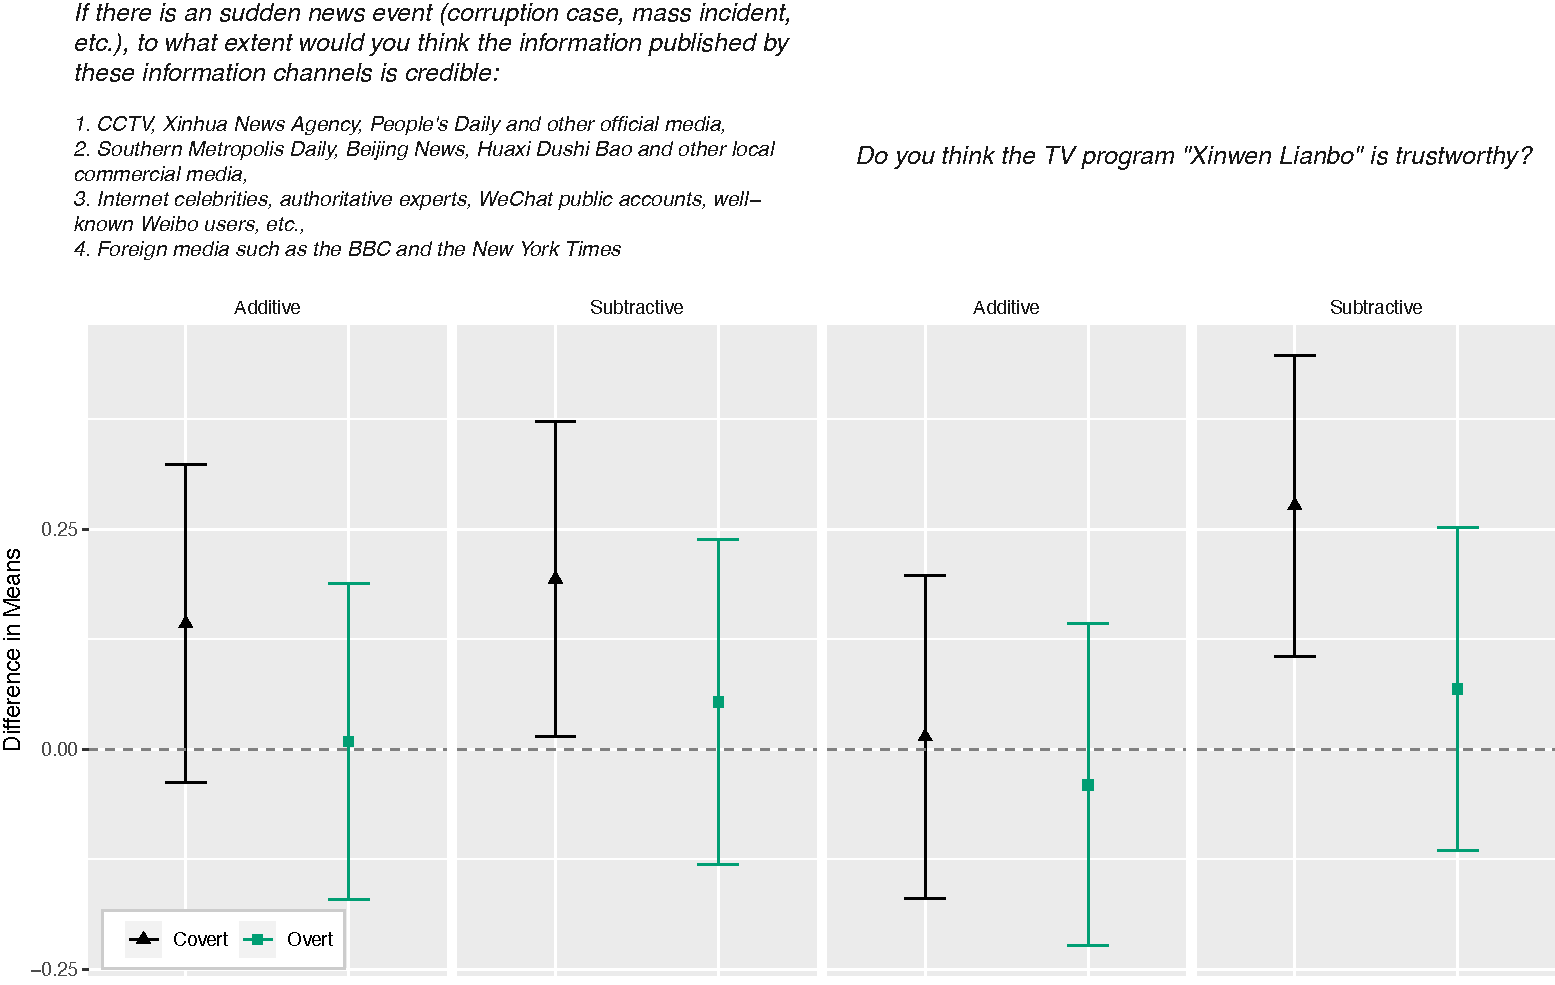
\includegraphics[width=.9\textwidth]{figures/raw_media_trust.pdf}\\
        \label{ATE_media_trust}
    \end{center}
    \vspace{1em}
\end{minipage}

Finally, I find evidence that overt additive information control can lead to poor user experience. According to two measures of user experience, I found that users expressed greater dissatisfaction with the platform when information control was covert. In addition, I also find that covert treatments increase user experience when compared to overt treatments (see \hyperref[ATE_ux]{Figure \ref*{ATE_ux}}).

\begin{minipage}{\linewidth}
    \vspace{3em}
    \begin{center}
  		\captionof{figure}{User Experience Measures for the Additive Treatment Group}
        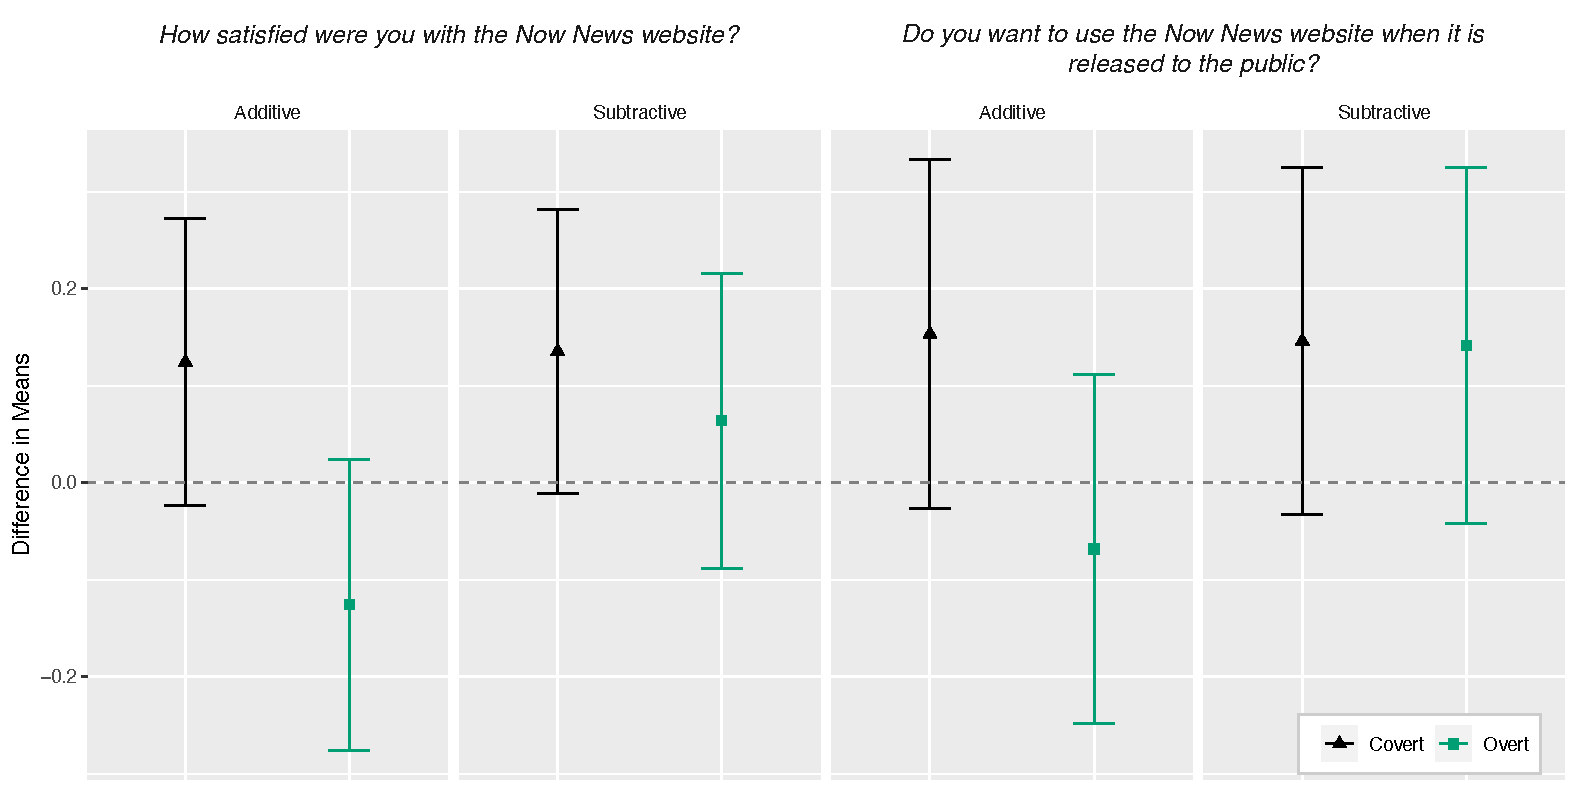
\includegraphics[width=.9\textwidth]{figures/raw_ux.pdf}\\
        \label{ATE_ux}
    \end{center}
    \vspace{1em}
\end{minipage}

Additive and subtractive information control conditions significantly decreased subjects perceptions of discourse competition in the comment section (see \hyperref[ATE_discourse_comp]{Figure \ref*{ATE_discourse_comp}}). As expected, users perceived lower discourse competition in the subtractive treatment than in the additive treatment (hypothesis 3). And as there were no changes to the distribution of comments in the suppressive treatment, there was no observed effect on discourse competition compared to the baseline.

\begin{minipage}{\linewidth}
    \begin{center}
  		\captionof{figure}{Perceptions of Discourse Competition by Treatment Group}
        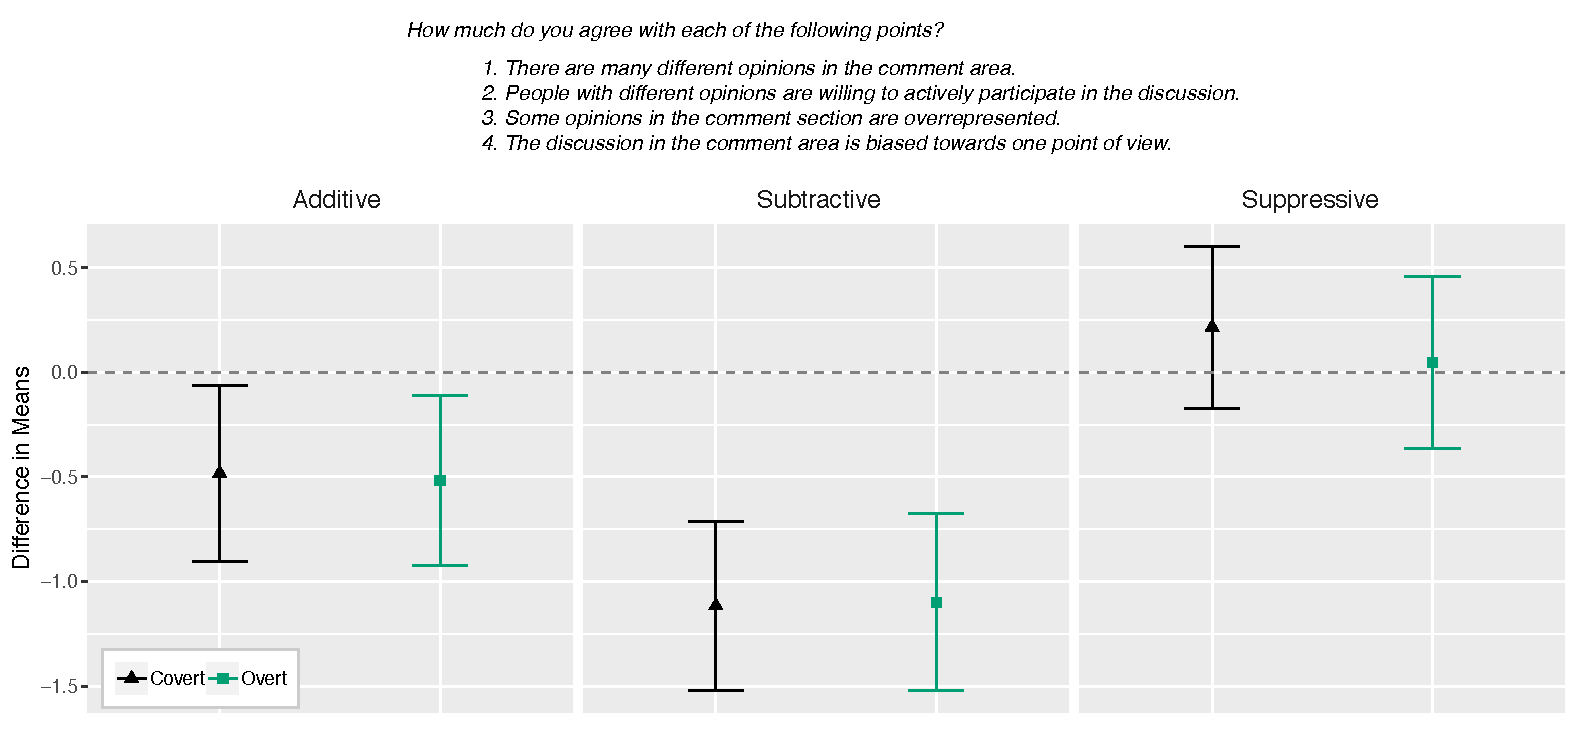
\includegraphics[width=.9\textwidth]{figures/ATE_discourse_comp.pdf}\\
        \label{ATE_discourse_comp}
    \end{center}
    \vspace{.5em}
\end{minipage}

While I sought to test heterogeneous effects, problems with data collection (likely due to the political sensitivity of the survey) left me with a smaller sample size than I originally intended. Because of this, there is not enough power to report results for heterogeneous effects.

\section{Conclusion}\label{conclusion}

In this paper I introduce the strategy of informational repression in the Chinese context. The strategy of informational repression combines digital surveillance and covert forms of repression to achieve social compliance while limiting the scope and visibility of the states repressive tactics. I argue that informational repression limits backlash against the state and ICTs, while preserving the appearance of discourse competition online, resulting in a more-reliable source of information needed to respond to threats. I traced the process of state-ICT contestation that has led to this strategy. I then reviewed government documents and public statements that demonstrate a move to concentrate specifically on social influence.

To illustrate how covert information control can benefit both the state and ICTs, I conducted an online experiment with Chinese internet users. I found that covert tactics benefit both the government and private companies, as users in the covert treatment groups had appreciably more favorable views of state media and their experience on a fictional news aggregator site. Furthermore, I also demonstrated that covert tactics gave users a greater impression of discourse competition on the fictional platform. This suggests that covert information control can also give individuals a sense that the opinions they observe are representative, and that there is less intervention online. In sum, information control mitigates the threat of virality while also limiting backlash and chilling effects that can result from heavy-handed censorship.


\newpage

\section{Appendix}\label{appendix}

\subsection{Article Text}\label{text}

\subsubsection{English}

Title: Timely Amend Internet-Based Ride-Share Policy\newline

\noindent Global Times Opinion: March 8, 2018 9:20 AM\newline

The internet-based ride-share policy has entered the full implementation stage. The policy is a major innovation and reform.

Internet-based ride-share services, as a classic model in the internet economy, is unique due to its cross-regional operations, which requires each locale to be innovative and flexible with their policies. However, the strictly local governance of the industry means that the cost of repeated auditing increases heavily and brings unnecessary burden to the services.

The internet-based ride-share policy is established to address these burdens and encourage the industry’s development. Therefore, local governments should reasonably relax their implementation policies in order to provide convenience transportation for passengers and counteract illegal taxi services by creating a sound resolution mechanism.

The internet-based ride-share policy aims to resolve safety problems and ensure the passengers’ legal rights by establishing a comprehensive mechanism that includes establishing barriers to entry on vehicle hardware, providing adequate insurance policies to drivers and ensuring rideshare services take more responsibility for vehicle safety.

Through a positive and cooperative mechanism which includes the government, the corporations, and the society, the remaining issues could be resolved.

\subsubsection{Mandarin}

\begin{minipage}{\linewidth}

\zh{适时给网约车政策打补丁}\newline

\noindent\zh{2018年03月08日 09:20 环球时报评论}\newline

\zh{网约车政策进入全面正式实施阶段,其制定是一场制度创新与改革。作为网络经济的一种典型模式,网约车有着跨地域经营的特点。因此,对属地管理制度要求灵活创新。但是,严格的属地管理特点意味着增加了各属地重复审核的行政成本,为网约车行业带来不必要的政策壁垒。}

\zh{网约车政策目的在于打破政策壁垒、鼓励行业发展。各地方的实施细应当适度松开政策口袋,在解决出行难的同时进一步改善经营管理,通过建立合理的疏导机制,统筹解决黑车这一社会顽疾。}

\zh{网约车政策也重点解决安全问题,通过建立一套完整的机制,包括对于车辆硬件建立准入门槛、设置合理的保险制度、明晰平台的责任等方式保障乘客合法权益。}

\zh{深化网约车行业管理体制改革,需要进一步拓宽思路,通过良性的制度设计以及政企合作、社会共治的模式来解决问题。}

\end{minipage}

\subsection{Comment Interface}
\vspace{-2em}
\begin{table}[H]
  \singlespacing
  \centering
  \caption{Ordinary Avatars}
  \begin{tabular}{|p{.125\textwidth}|p{.2\textwidth}|p{.45\textwidth}|p{.1\textwidth}|}
	\hline
	\textbf{Gender} & \textbf{Username} & \textbf{Username (English)} & \textbf{Avatar} \\ \hline
	Female & \zh{芽雅92} & Elegant Sprout 92 & \begin{minipage}{.2\textwidth}
\includegraphics[width=.45\linewidth, height=.45\linewidth]{figures/ordinary_avatars/f1.jpg}\end{minipage} \\ \hline
	Female & \zh{爱粽子的蚊子} & Dumpling-loving Mosquito & \begin{minipage}{.2\textwidth}
\includegraphics[width=.45\linewidth, height=.45\linewidth]{figures/ordinary_avatars/f2.jpg}\end{minipage} \\ \hline
	Female & \zh{老丸子89} & Old Meatball 89 & \begin{minipage}{.2\textwidth}
\includegraphics[width=.45\linewidth, height=.45\linewidth]{figures/ordinary_avatars/f3.jpg}\end{minipage} \\ \hline
	Female & \zh{雅思精解} & Elegant, thoughtful, energetic, liberated & \begin{minipage}{.2\textwidth}
\includegraphics[width=.45\linewidth, height=.45\linewidth]{figures/ordinary_avatars/f4.jpg}\end{minipage} \\ \hline
	Female & \zh{康尼岛大盗} & Coney Island Bandit & \begin{minipage}{.2\textwidth}
\includegraphics[width=.45\linewidth, height=.45\linewidth]{figures/ordinary_avatars/f5.jpg}\end{minipage} \\ \hline
	Female & \zh{等你的兔子} & Wait for your rabbit & \begin{minipage}{.2\textwidth}
\includegraphics[width=.45\linewidth, height=.45\linewidth]{figures/ordinary_avatars/f6.jpg}\end{minipage} \\ \hline
	Male & \zh{我心本尊} & Respect at the bottom of my heart & \begin{minipage}{.2\textwidth}
\includegraphics[width=.45\linewidth, height=.45\linewidth]{figures/ordinary_avatars/m1.jpg}\end{minipage} \\ \hline
	Male & \zh{章鱼丸子} & Octopus meatballs & \begin{minipage}{.2\textwidth}
\includegraphics[width=.45\linewidth, height=.45\linewidth]{figures/ordinary_avatars/m2.jpg}\end{minipage} \\ \hline
	Male & \zh{奇幻雨林} & Magical Rainforest & \begin{minipage}{.2\textwidth}
\includegraphics[width=.45\linewidth, height=.45\linewidth]{figures/ordinary_avatars/m3.jpg}\end{minipage} \\ \hline
	Male & \zh{那小子真帅44} & That guy is really handsome 44 & \begin{minipage}{.2\textwidth}
\includegraphics[width=.45\linewidth, height=.45\linewidth]{figures/ordinary_avatars/m4.jpg}\end{minipage} \\ \hline
	Male & \zh{太阳之光82} & Sunlight 82 & \begin{minipage}{.2\textwidth}
\includegraphics[width=.45\linewidth, height=.45\linewidth]{figures/ordinary_avatars/m5.jpg}\end{minipage} \\ \hline
	Male & \zh{萌面小怪兽} & Cute-faced Little Monster & \begin{minipage}{.2\textwidth}
\includegraphics[width=.45\linewidth, height=.45\linewidth]{figures/ordinary_avatars/m6.jpg}\end{minipage} \\ \hline
	Unspecified & \zh{爱玩的小胖} & Playful chubby thing & \begin{minipage}{.2\textwidth}
\includegraphics[width=.45\linewidth, height=.45\linewidth]{figures/ordinary_avatars/o1.jpg}\end{minipage} \\ \hline
	Unspecified & \zh{好人520} & Good person 520 (I love you) & \begin{minipage}{.2\textwidth}
\includegraphics[width=.45\linewidth, height=.45\linewidth]{figures/ordinary_avatars/o2.jpg}\end{minipage} \\ \hline
	Unspecified & \zh{可保平安} & Safe and sound & \begin{minipage}{.2\textwidth}
\includegraphics[width=.45\linewidth, height=.45\linewidth]{figures/ordinary_avatars/o3.jpg}\end{minipage} \\ \hline
  \end{tabular}
  \label{uids}
\end{table}

\begin{table}[H]
  \singlespacing
  \centering
  \caption{Government Avatars}
  \begin{tabular}{|p{.125\textwidth}|p{.2\textwidth}|p{.45\textwidth}|p{.1\textwidth}|}
	\hline
	\textbf{Gender} & \textbf{Username} & \textbf{Username (English)} & \textbf{Avatar} \\ \hline
	Unspecified & \zh{上海交警} & Shanghai Traffic Police & \begin{minipage}{.2\textwidth}
\includegraphics[width=.5\linewidth, height=.5\linewidth]{figures/govt_avatars/1.jpg}\end{minipage} \\ \hline
	Unspecified & \zh{上海交警网评员} & Shanghai Traffic Police commentator & \begin{minipage}{.2\textwidth}
\includegraphics[width=.5\linewidth, height=.5\linewidth]{figures/govt_avatars/2.jpg}\end{minipage} \\ \hline
	Unspecified & \zh{上海发布网评员} & Shanghai Publicity commentator & \begin{minipage}{.2\textwidth}
\includegraphics[width=.5\linewidth, height=.5\linewidth]{figures/govt_avatars/3.jpg}\end{minipage} \\ \hline
	Female & \zh{上海胡警官} & Shanghai Police Officer Hu & \begin{minipage}{.2\textwidth}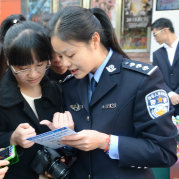
\includegraphics[width=.5\linewidth, height=.5\linewidth]{figures/govt_avatars/4.jpg}\end{minipage} \\ \hline
	Unspecified & \zh{中山民众镇青年志愿者} & Zhongshan Township Youth Volunteers & \begin{minipage}{.2\textwidth}
\includegraphics[width=.5\linewidth, height=.5\linewidth]{figures/govt_avatars/5.jpg}\end{minipage} \\ \hline
	Male & \zh{上海林警官} & Shanghai Police Officer Lin & \begin{minipage}{.2\textwidth}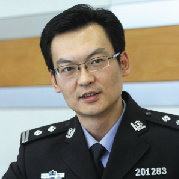
\includegraphics[width=.5\linewidth, height=.5\linewidth]{figures/govt_avatars/6.jpg}\end{minipage} \\ \hline
  \end{tabular}
  \label{uidgov}
\end{table}

\begin{table}[H]
    \singlespacing
    \centering
    \singlespacing
    \caption{All Comments}
    \label{comments}
    \resizebox{\textwidth}{!}{
    \begin{tabular}{|p{.14\textwidth}|p{.52\textwidth}|p{.28\textwidth}|p{.1\textwidth}|}
    \hline
        \textbf{Type} & \textbf{English} & \textbf{Chinese} & \textbf{Position} \\ \hline
        Critical & Isn't this kind of regulation is essentially prohibiting ride-share services? & \zh{这样管理还不如直接禁止网约车算了}  & 2 \\ \hline
        Critical & The number of illegal taxis in Shanghai never decreases. Damn. The authorities are all idling about. & \zh{上海的黑车什么时候少过 册那 管事的都是游手好闲。} & 12 \\ \hline
        Critical & Strict legislation, prevalent violation, selective enforcement, what's expected from the Communist Party.  & \zh{严格立法,普遍违法,选择执法,共党日常} & 13 \\ \hline
        Neutral & Ride-sharing cars need to display a sign, just like taxis do. It's easier for traffic police to supervise them this way. & \zh{网约车也要象的士一样,挂上标识,标注网约车三个字,方便交警管理。}  & 6 \\ \hline
        Neutral & The emergence of ride-sharing services reflects the development of the times. The emergence of a new industry certainly will come with lots of problems. The point is how to solve these problems.  & \zh{网约车是顺应时代发展的产物,一个新型行业的出现,必然会伴随很多问题,怎么处理好这些问题才是关键 } & 9 \\ \hline
        Neutral & I'd like to make a policy suggestion: passengers should be allowed to keep drivers' cell phones while they are in a taxi or using the Internet-based ride-share services like DIDI. Eight out of ten drivers are using their phones while driving. They don't even notice the traffic light when it turns green. & \zh{实名建议出台政策允许乘客打出租车或者滴滴这类的网约车时有权暂时替司机保管手机 十个司机里面八个边玩手机边开车 信号灯转绿了都不知道 } \hspace{.25em} 
\includegraphics[width=1.25em]{figures/emoji.png}& 15 \\ \hline
        Support & Support companies, support the economy, support reform, realize revitalization! & \zh{支持企业,发展经济,促进改革,实现振兴!}  & 1 \\ \hline
        Support & This policy will help the healthy development of the ride-sharing industry! & \zh{这个政策会推动网约车行业的健康发展!}  & 3 \\ \hline
        Support & Thank you Central Government for the good policy & \zh{感谢中央的好政策}  & 7 \\ \hline
        Astroturfing & The care for people from the Party and the nation is the warmest thing. & \zh{最给人温暖的,源自党和国家对人民的关怀。}  & 4 \\ \hline
        Astroturfing & The Party's policies are getting better and better, China's future will inevitably be bright. & \zh{党的政策越来越好,中国的未来必将更加美好 } & 5 \\ \hline
        Astroturfing & Listen to the Party and follow the Party! & \zh{听党话,跟党走!} & 8 \\ \hline
        Astroturfing & So many good policies make people full of hope for the future. & \zh{一项项利好政策的出台让人民对未来充满希望。} & 10 \\ \hline
        Astroturfing & Our country has introduced another policy that reflects a good deal of consultation [with the people]. & \zh{国家多出台一些像若干意见这些的政策。} & 11 \\ \hline
        Astroturfing & I hope that even more favorable policies are introduced to bring benefits to the people. & \zh{希望有更多优惠政策出台,让老百姓受益。} & 14 \\ \hline
    \end{tabular}
    }
\end{table}

\subsection{Survey Questionnaire}

\begin{table}[H]
    \singlespacing
    \centering
    \caption{Pre-Treatment Questions}
    \label{pre_treatment}
    \resizebox{\textwidth}{!}{
    \begin{tabular}{|c|p{.25\textwidth}|p{.45\textwidth}|p{.35\textwidth}|p{.18\textwidth}|}
    \hline
        \textbf{\#} & \textbf{Purpose} & \textbf{Question (EN)} & \textbf{Question (ZH)} & \textbf{Variable Type} \\\hline
        Q1 & Human Subjects Statement & - & - & - \\\hline
        Q2 & Browser Metadata & - & - & - \\\hline
        Q3 & Age & In what year were you born? & \zh{请问您是哪年出生的?} & Integer (1900-2001) \\\hline
        Q4 & Gender & What is your gender? & \zh{您的性别为:} & M, F, Other \\\hline
        Q5 & Province & In which province do you live? & \zh{您目前居住在哪个省?} & Multiple Choice \\\hline
        Q6 & Hukou & What type of hukou do you have? & \zh{您的户口为农业户口还是非农业户口?} & Urban/Rural \\\hline
        Q7 & Ethnicity & What ethnicity is on your identity card? & \zh{您属于哪个民族?(以身份证信息为准)} & Multiple Choice \\\hline
        Q8 & Years of education & How many years of education have you received? & \zh{您接受过多少年教育?} & Positive Integer \\\hline
        Q9 & Work Unit & In your career, what kind of work units have you been employed by? & \zh{您是否在以下这些类单位工作过?} & Multiple Choice \\\hline
        Q10 & Ideology & As a news media organization, we aim to provide our readers with the most trustworthy news sources. Generally speaking, what is your level of trust of these types of news sources? (central government official, entrepreneur, government official, doctor, banking executive, ordinary person, firefighter, university student) & \zh{作为一家新闻公司,我们希望为您提供最可靠的信息涞源。总体来说,您对以下这几种信息涞源的信任程度是怎样? (中央政府官员、企业家、地方政府官员、医生、银行高管、普通老百姓、消防员、大学生)} & - \\\hline
        Q11 & Newspaper Exposure & During a typical week, how many days do you read news in a printed newspaper? & \zh{在过去的一周内,您有多少天通过纸质媒体阅读新闻?} & Integer (1-7) \\\hline
        Q12 & Newspaper Exposure & Which of the following newspapers have you read in the last month? & \zh{在过去的一个月内,您曾阅读过下列哪些报纸?} & Multiple Answer \\\hline
        Q13 & Television Exposure & During a typical week, how many days do you watch news on TV? & \zh{在过去的一周内,您有多少天通过电视观看新闻?} & Integer (1-7) \\\hline
        Q14 & Television Exposure & Which of the following television news programs have you watched in the last month? & \zh{在过去的一个月内,您曾观看过下列哪些新闻节目?} & Multiple Answer \\\hline
        Q15 & Internet News Exposure & During a typical week, how many days do you watch or read news on the Internet? & \zh{在过去的一周内,您有多少天通过互联网获取新闻?} & Integer (1-7) \\\hline
        Q16 & Internet News Exposure & Which of the following news websites have you visited in the last month? & \zh{在过去的一个月内,您曾访问过下列哪些新闻网站?} & Multiple Answer \\\hline
        Q17 & Social Media Exposure & During a typical week, how many days do you watch or read news on social media (i.e. Weibo, WeChat, QQ, etc.)? & \zh{在过去的一周内,您有多少天通过社交媒体(比如微信、微博、QQ、等)获取新闻?} & Integer (1-7) \\\hline
        Q18 & Social Media Exposure & Which of the following social networking platforms have you visited in the last month? & \zh{在过去的一个月内,您曾访问过下列哪些社交媒体平台?} & Multiple Answer \\\hline
        Q19 & Ideology (Xi Jinping App) & Which of the following apps have you downloaded? & \zh{您下载过以下哪些移动应用程序(APP)?} & Multiple Answer \\\hline
        Q20 & Block Explainer & The next few questions will test your understanding of past and present hot news events. The following questions range from very easy to very difficult. Please answer to the best of your ability and don't worry about getting every question right. & \zh{接下来的几个问题将测试您对过去和近期热点事件的了解程度。以下问题难度各异,请按照您所知道的情况回答,回答时不必担心正确率。} &  \\\hline
        Q21 & Political Knowledge & Where was the 2016 G20 Conference was held? & \zh{以下哪座城市是2016年G20峰会的举办地?} & Multiple Choice \\\hline
        Q22 & Political Knowledge & In what year did Hong Kong return to the motherland? & \zh{香港在哪一年回归祖国?} & Multiple Choice \\\hline
        Q23 & Political Knowledge & Which of the following political slogans were not created under President Xi Jinping's leadership? & \zh{以下哪个理念不是在习近平的领导下提出的?} & Multiple Choice \\\hline
        Q24 & Political Knowledge & Who was China's Premier from 2003-2013? (Wang Qishan, Li Keqiang, Xi Jinping, Hu Jintao, Wen Jiabao, Jiang Zemin) & \zh{下列哪位国家领导人曾在2003至2013年间担任中华人民共和国总理?} & Multiple Choice \\\hline
        Q25 & Political Knowledge & In 2017 China had a border conflict with which country? & \zh{中国曾在2017年与下列哪个国家发生过边界冲突?} & Multiple Choice \\\hline
        Q26 & Political Knowledge & Do you know the name of your provincial-level party secretary's name? & \zh{您是否知道您所住地区省(市、自治区)党委书记的名字?} & Yes, No \\\hline
        \end{tabular}
    }
\end{table}

\begin{table}[H]
    \singlespacing
    \centering
    \caption{Post-Treatment Questions}
    \label{post_treatment_1}
    \resizebox{\textwidth}{!}{
    \begin{tabular}{|c|p{.15\textwidth}|p{.48\textwidth}|p{.38\textwidth}|l|}
    \hline
        \textbf{\#} & \textbf{Purpose} & \textbf{Question (EN)} & \textbf{Question (ZH)} & \textbf{Variable Type} \\\hline
        Q29 & Distractor & How often do you make purchases on Taobao? & \zh{您在淘宝上购物的频率:} & Multiple Choice \\\hline
        Q30 & Agreement with Policy & We are very interested in your opinion. Could you please share with us your opinion about the new ride share policy? Please write two or more sentences. & \zh{我们对您的观点很感兴趣,请您与我们分享您有关网约车政策的观点。请您提供两句话以上的评价。} & Open-ended \\\hline
        Q31 & Agreement with Policy & Recall the article you just read. If you had to guess, what position would most of your peers take on the ride-share policy discussed in the article? (very strongly support, strongly support, support, oppose, strongly oppose, very strongly oppose) & \zh{结合您刚刚阅读的文章,请您做出以下猜测,您周围的人对文章中提到的网约车政策持有怎样的立场?} & Multiple Choice \\\hline
        Q32 & Agreement with Policy & Recall the article you just read. What is your position on the ride-share policy discussed in the article? (very strongly support, strongly support, support, neutral, oppose, strongly oppose, very strongly oppose) & \zh{结合您刚刚阅读的文章,您对文章中提到的网约车政策持有怎样的立场?} & Multiple Choice \\\hline
        Q33 & Self-expression & How willing are you to post your opinion about this article on social media? (very unwilling, unwilling, slightly unwilling, neutral, slightly willing, willing, very willing) & \zh{您是否愿意将您对此文章的观点发布在社交媒体上?} & Multiple Choice \\\hline
        Q34 & Self-expression & How likely are you to state your opinion on ridesharing policy to a group of colleagues or friends if the topic came up in conversation? (very likely, likely, somewhat likely, neutral, somewhat unlikely, likely, very likely) & \zh{如果有人在谈话中提起此话题,你有多大可能向同事或朋友陈述你对网约车政策的意见?} & Multiple Choice \\\hline
        Q35 & Credibility & The opinions on the ride-share policy in the comment section are generally representative of the opinions held by society at large. & \zh{评论区的各种意见总体代表了社会对网约车的意见。} & Multiple Choice \\\hline
        Q36 & Discourse Competition & How much do you agree with each of the following points? 1) There are many different opinions in the comment area. 2) People with different opinions are willing to actively participate in the discussion. 3) Some opinions in the comment section are overrepresented. 4) The discussion in the comment area is biased towards one point of view. & \zh{请问您在多大程度上同意下面的观点:1)评论区有许多不同的观点。2)持有不同观点的人愿意积极参与讨论。3)某些意见在评论区中过多。4)评论区的讨论偏向于一个观点。} & Multiple Choice \\\hline
        Q37 & Discourse Competition/Credibility & Please share a bit about your experience with the article's comment area. Please write two or more sentences. & \zh{请您分享一下您对文章评论区域的阅读与使用体验。请您提供两句话以上的评价。} & Open-ended \\\hline
        Q38 & Block Explainer & Some readers prefer to read articles from Party media outlets while others prefer more independent media outlets. This section will help us understand how to best serve each type of reader. & \zh{有些读者喜欢阅读官媒的新闻,而有些读者更喜欢阅读商业媒体的新闻。 接下来这部分调查是关于您的阅读偏好。} & - \\\hline
        Q39 & Trust in State Media & Do you think the TV program ``Xinwen Lianbo'' is trustworthy? (very trustworthy, trustworthy, somewhat trustworthy, neutral, somewhat untrustworthy, untrustworthy, very untrustworthy) & \zh{您认为《新闻联播》节目内容可信度如何?} & Multiple Choice \\\hline
        Q40 & Trust in State Media & If there is an sudden news event (corruption case, mass incident, etc.), to what extent would you think the information published by these information channels is credible: 1) CCTV, Xinhua News Agency, People's Daily and other official media, 2) Southern Metropolis Daily, Beijing News, Huaxi Dushi Bao and other local commercial media, 3) Internet celebrities, authoritative experts, WeChat public accounts, well-known Weibo users, etc., 4) Foreign media such as the BBC and the New York Times & \zh{假如发生突发事件(腐败案件、群体性事件等),下面这些信息渠道发布的信息您在多大程度上觉得可信?1) 央视、新华社、人民日报等官方媒体, 2) 南方都市报、新京报、华西都市报等地方性商业媒体, 3) 网络名人、权威专家的微信公众号、知名微博等自媒体, 4) BBC、纽约时报等国外媒体} & Multiple Choice \\\hline
    \end{tabular}
    }
\end{table}

\begin{table}[H]
    \singlespacing
    \caption{Post-Treatment Questions (continued)}
    \label{post_treatment_2}
    \resizebox{\textwidth}{!}{
    \begin{tabular}{|c|p{.18\textwidth}|p{.52\textwidth}|p{.4\textwidth}|p{.12\textwidth}|}
    \hline
        \textbf{\#} & \textbf{Purpose} & \textbf{Question (EN)} & \textbf{Question (ZH)} & \textbf{Variable Type} \\\hline
        Q41 & Trust in State Media & Could you please explain your answers to the previous two questions? & \zh{您能解释一下您对前两个问题的答案吗?请您提供两句话以上的评价。} & Open-ended \\\hline
        Q42 & Legitimacy & Do you agree with the following: ``Our government is working for the people and serving their needs'' (strongly agree, agree, somewhat agree, neutral, somewhat disagree, disagree, very much disagree) & \zh{您同意下列说法吗?``总的来说,我们的政府在响应人民的要求,为人民做事。}'' & Multiple Choice \\\hline
        Q43 & Legitimacy & How do you feel about the current status quo in China? (very satisfied, satisfied, somewhat satisfied, neutral, somewhat dissatisfied, dissatisfied, very dissatisfied) & \zh{您对中国目前总体现状感觉如何?}  & Multiple Choice \\\hline
        Q44 & Legitimacy & Could you please explain your answers to the previous two questions? Please write two or more sentences. & \zh{您能解释一下您对前两个问题的答案吗?请您提供两句话以上的评价。} & Open-ended \\\hline
        Q45 & Block Explainer & In order to improve our products as much as possible, we invite you to answer the following questions about your user experience. Any suggestions you have will be incredibly helpful to us, thank you for your sincere feedback. & \zh{为了尽可能优化我们的产品, 我们诚邀您对以下使用体验问题进行回答。您的任何反馈都将会为我们提供巨大的帮助,感谢您的真诚反馈。} & - \\\hline
        Q46 & User Satisfaction & How satisfied were you with the Now News website? (Very satisfied, satisfied, somewhat satisfied, neutral, somewhat unsatisfied, unsatisfied, very unsatisfied) & \zh{您对Now新闻网的满意程度:} & Multiple Choice \\\hline
        Q47 & User Satisfaction & Do you want to use the Now News website when it is released to the public? (Really want to use, want to use, somewhat want to use, indifferent, somewhat don't want to use, don't want to use, really do not want to use) & \zh{在Now新闻正式发布时,您是否想使用这个网站?} & Multiple Choice \\\hline
        Q48 & User Satisfaction & Could you explain in a few sentences your answers to the previous two questions? &\zh{您能解释一下您对前两个问题的答案吗?请您提供两句话以上的评价。} & Open-ended \\\hline
        Q49 & Block Explainer & Readers have many different perspectives on international politics. This section will help us understand how to provide a wide range of perspectives to each type of reader. & \zh{在我们的新闻报道中包含了许多有关国际关系的观点。作为一个对读者来说十分重要的话题,我们将在下一部分的调查中就中国的国际关系向您提出一些问题。} & - \\\hline
        Q50 & Nationalism & How much do you agree with each of the following statements: 1) Even if I could choose any other country in the world, I would prefer to be a citizen of China than any other country, 2) In general, China is a better country than most others, 3) Whenever someone criticizes China, I feel like they are criticizing me. & \zh{请问您在多大程度上同意下面的观点:1)即使可以选择世界上任何国家,我也更愿意做中国公民。2)总的来说,中国比其他大部分国家都好。3)别人批评中国时,就像在批评我自己} & Multiple Choice \\\hline
        Q51 & Nationalism & Could you please explain your answers to the previous question? Please write two or more sentences. & \zh{您能解释一下您对上一个问题的答案吗?请您提供三句话以上的评价。}  & Open-ended \\\hline
        Q52 & Distractor & Which of the following mobile operating systems do you use? & \zh{您使用以下哪种手机操作系统?} & Multiple Choice \\\hline
        Q53 & Collective Action & How likely are you to sign a petition to support something you highly in favor of? (very likely, likely, somewhat likely, neutral, somewhat unlikely, likely, very likely) & \zh{您有多大可能会通过联名上书来表达您的观点和信念?} & Multiple Choice \\\hline
        Q54 & Collective Action & How likely are you to join a petition to support something you are highly in favor of? (very likely, likely, somewhat likely, neutral, somewhat unlikely, likely, very likely) & \zh{您有多大可能会通过参加信访、上访来表达您的观点和信念?} & Multiple Choice \\\hline
        Q55 & Collective Action & How likely are you to join a march to support something you are highly in favor of? (very likely, likely, somewhat likely, neutral, somewhat unlikely, likely, very likely) & \zh{您有多大可能会通过参加游行集会来表达您的观点和信念?} & Multiple Choice \\\hline
        Q56 & Collective Action & Could you explain in a few sentences your answers to the previous three questions? & \zh{您能解释一下您对前三个问题的答案吗?请您提供三句话以上的评价。 }& Open-ended \\\hline
    \end{tabular}
    }
\end{table}

\begin{table}[H]
    \singlespacing
    \centering
    \caption{Manipulation and Attention Checks}
    \label{manip_check}
    \resizebox{\textwidth}{!}{
    \begin{tabular}{|c|p{.15\textwidth}|p{.45\textwidth}|p{.35\textwidth}|l|}
    \hline
        \textbf{\#} & \textbf{Purpose} & \textbf{Question (EN)} & \textbf{Question (ZH)} & \textbf{Variable Type} \\\hline
        Q57 & Manipulation & Which notice below was displayed in the comment area? & \zh{评论区中出现过哪个通知?} & Multiple Choice \\\hline
        Q58 & Manipulation Check & Were there any comments on the official account of the party and government agencies (such as the public security bureau, the Communist Youth League, etc.) in the comment area (with the V logo)? & \zh{在评论区中有没有经过认证的党政机关(例如公安、共青团、等)官方账号(带有V标志)的评论?} & Multiple Choice \\\hline
        Q59 & Attention & What is the topic of this article? & \zh{这篇报道的主题是什么?} & Multiple Choice \\\hline
        Q60 & Attention & The price of the ride-sharing services and taxis may be different. We want to know your point of view. To prove that you are paying attention, please choose the third answer: & \zh{网约车和出租车的价格可能不同,我们想知道您的观点。为了证明您正在关注,请选择第三个答案:} & Multiple Choice \\\hline
        Q61 & Attention & Was this image displayed in the article? & \zh{文章中是否出现过该图片?} & Multiple Choice \\\hline
        Q62 & Manipulation & If you had to guess, how many comments in the comment section of the article were in favor of the ride-share policy? & \zh{请您做出猜测,文章的评论区有多少赞成网约车政策的评论?} & Multiple Choice \\\hline
    \end{tabular}
    }
\end{table}


\begin{table}[H]
  \singlespacing
  \centering
  \caption{Media Exposure Sources}
  \resizebox{\textwidth}{!}{
  \begin{tabular}{|c|c|c|c|}
	\hline
		\textbf{Name (ZH)} & \textbf{Name (EN)} & \textbf{Source Type} & \textbf{Medium} \\ \hline
        \zh{参考消息} & Reference News & Semiofficial & Newspaper \\ \hline
        \zh{经济日报} & Economic Daily & Semiofficial & Newspaper \\ \hline
        \zh{华商报} & Chinese Business Paper & Semiofficial & Newspaper \\ \hline
        \zh{人民日报} & People's Daily & Official & Newspaper \\ \hline
        \zh{工人日报} & Workers' Daily & Official & Newspaper \\ \hline
        \zh{环球时报} & Global Times & Official & Newspaper \\ \hline
        \zh{经济观察报} & Economic Observer & Commercialized & Newspaper \\ \hline
        \zh{21世纪经济报道} & 21st Century Economic Report & Commercialized & Newspaper \\ \hline
        \zh{财经时报} & Business Times & Commercialized & Newspaper \\ \hline
        \zh{人民网} & People's Network & Official & Website \\ \hline
        \zh{央视网} & CCTV & Official & Website \\ \hline
        \zh{新华网} & xinhuanet & Official & Website \\ \hline
        \zh{网易新闻} & NetEase & Commercialized & Website \\ \hline
        \zh{新浪新闻} & Sina News & Commercialized & Website \\ \hline
        \zh{今日头条} & Toutiao & Commercialized & Website \\ \hline
        \zh{腾讯新闻} & Tencent News & Commercialized & Website \\ \hline
        \zh{搜狐新闻} & Sohu News & Commercialized & Website \\ \hline
        \zh{凤凰网} & Phoenix News & Commercialized & Website \\ \hline
        \zh{纽约时报} & The New York Times & Blocked & Website \\ \hline
        \zh{明报新闻网} & Mingpao & Blocked & Website \\ \hline
        \zh{苹果日报} & Apple Daily & Blocked & Website \\ \hline
        \zh{微信} & WeChat & Domestic & Social Media Platform \\ \hline
        \zh{新浪微博} & Sina Weibo & Domestic & Social Media Platform \\ \hline
        \zh{腾讯QQ} & Tencent QQ & Domestic & Social Media Platform \\ \hline
        \zh{百度贴吧} & Baidu Tieba & Domestic & Social Media Platform \\ \hline
        \zh{豆瓣} & Douban & Domestic & Social Media Platform \\ \hline
        \zh{知乎} & Zhihu & Domestic & Social Media Platform \\ \hline
        \zh{Facebook (脸书)} & Facebook & Blocked & Social Media Platform \\ \hline
        \zh{Twitter (推特)} & Twitter & Blocked & Social Media Platform \\ \hline
        \zh{Instagram} & Instagram & Blocked & Social Media Platform \\ \hline
        \zh{新闻联播} & Xīnwén Liánbò & - & Television Program \\ \hline
        \zh{焦点访谈} & Jiāodiǎn Gǎngtán & - & Television Program \\ \hline
        \zh{今日关注} & Jīnrì Guānzhù & - & Television Program \\ \hline
        \zh{海峡两岸} & Hǎixiá Liǎng'àn & - & Television Program \\ \hline
        \zh{新闻30分} & Xīnwén 30 Fēn & - & Television Program \\ \hline
        \zh{中国新闻} & Zhōngguó Xīnwén & - & Television Program \\ \hline
        \zh{今日亚洲} & Jīnrì Yàzhōu & - & Television Program \\ \hline
        \zh{中国舆论场} & Zhōngguó Yúlùn Chǎng & - & Television Program \\ \hline
        \zh{深度国际} & Shēndù Guójì & - & Television Program \\ \hline
  \end{tabular}
  }
  \label{exposure}
\end{table}

\subsection{Coding Diagrams for Comments and Open-Ended Responses}\label{diags}

\begin{figure}
  \centering
  \caption{Collective Action Coding Diagram}
  \vspace{1em}
  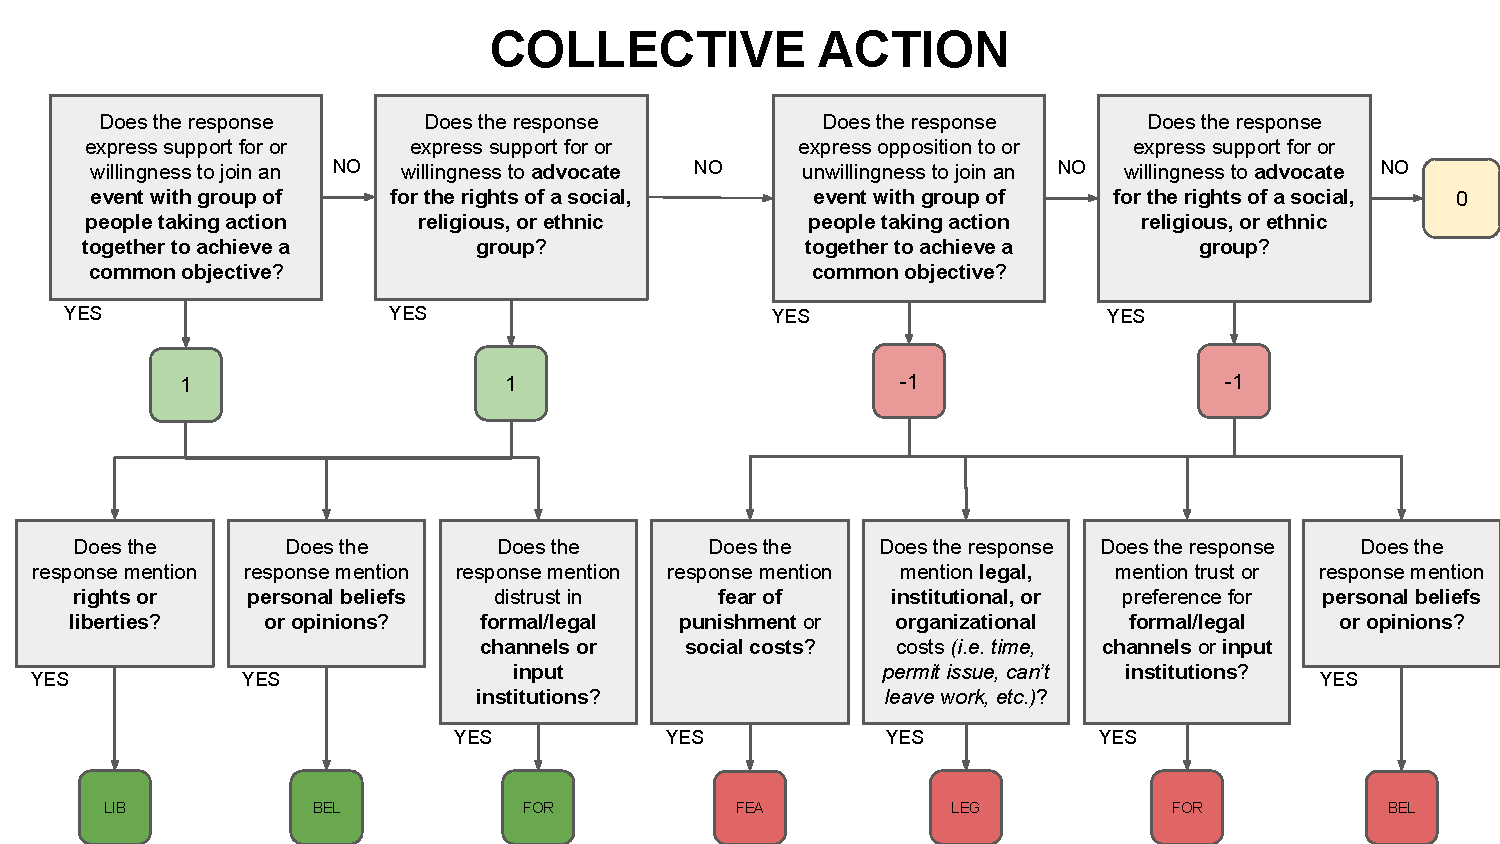
\includegraphics[width=\textwidth]{figures/coding_diagrams/collective_action.pdf}
  \label{collective_action}
\end{figure}

\begin{figure}
  \centering
  \caption{Legitimacy Coding Diagram}
  \vspace{1em}
  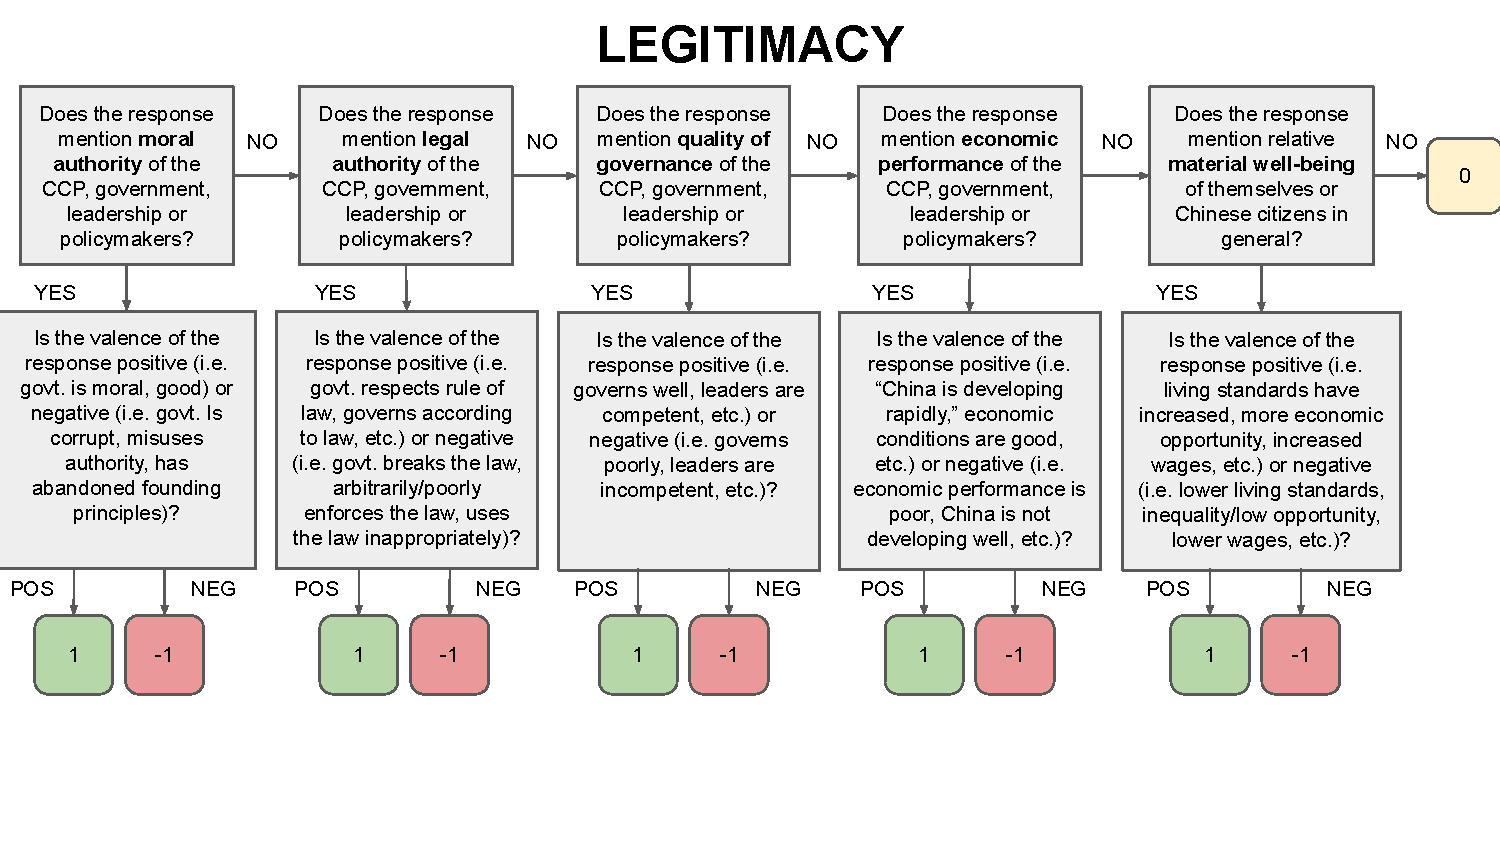
\includegraphics[width=\textwidth]{figures/coding_diagrams/legitimacy.pdf}
  \label{legitimacy}
\end{figure}

\begin{figure}
  \centering
  \caption{User Satisfaction and State Media Affinity Coding Diagrams}
  \vspace{1em}
  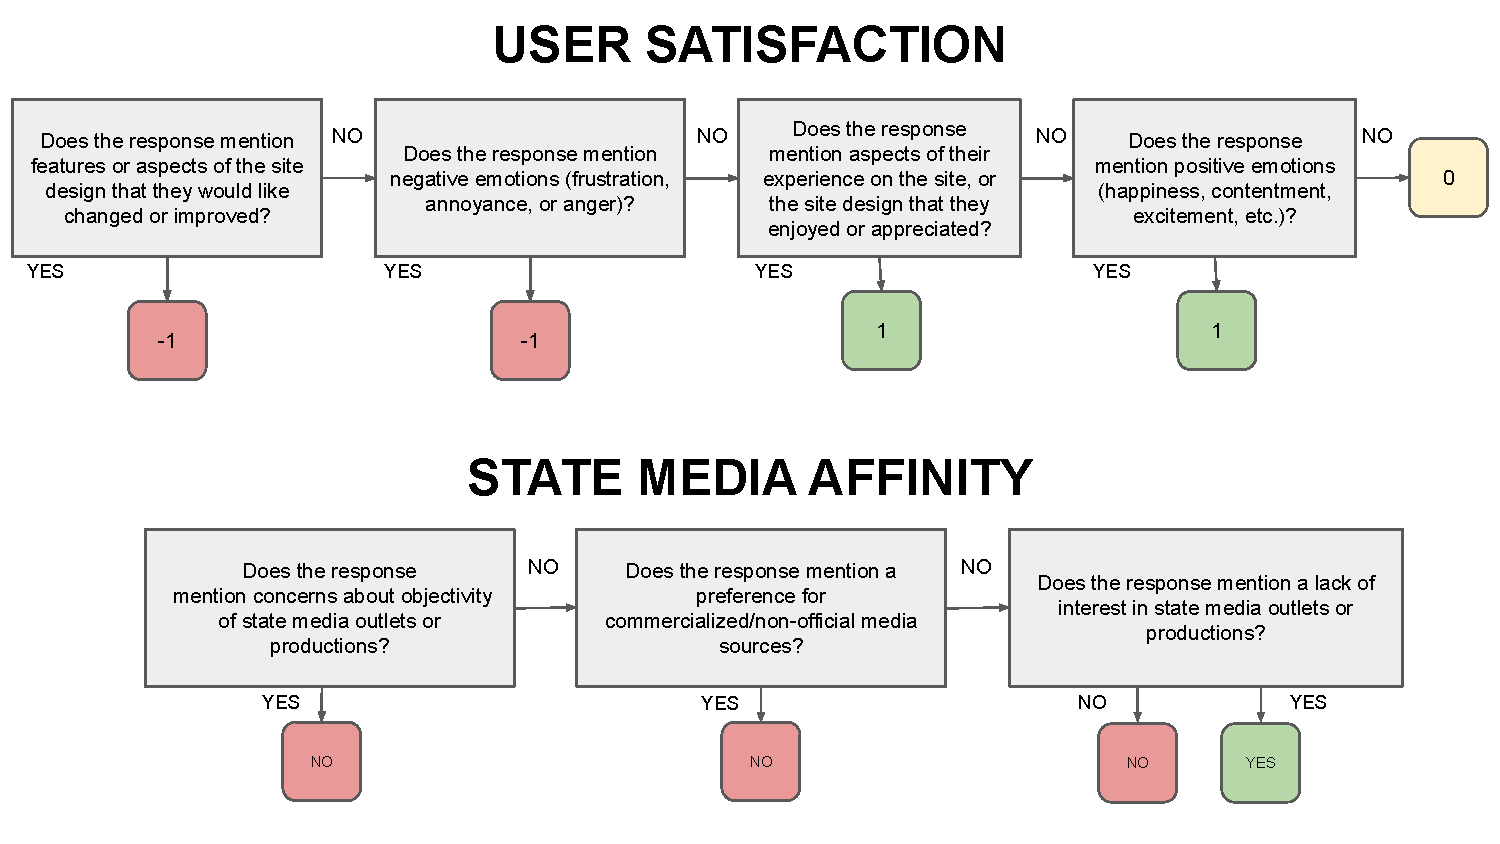
\includegraphics[width=\textwidth]{figures/coding_diagrams/user_sat_state_media.pdf}
  \label{user_sat_state_media}
\end{figure}

\begin{figure}
  \centering
  \caption{Favorability Coding Diagram}
  \vspace{1em}
  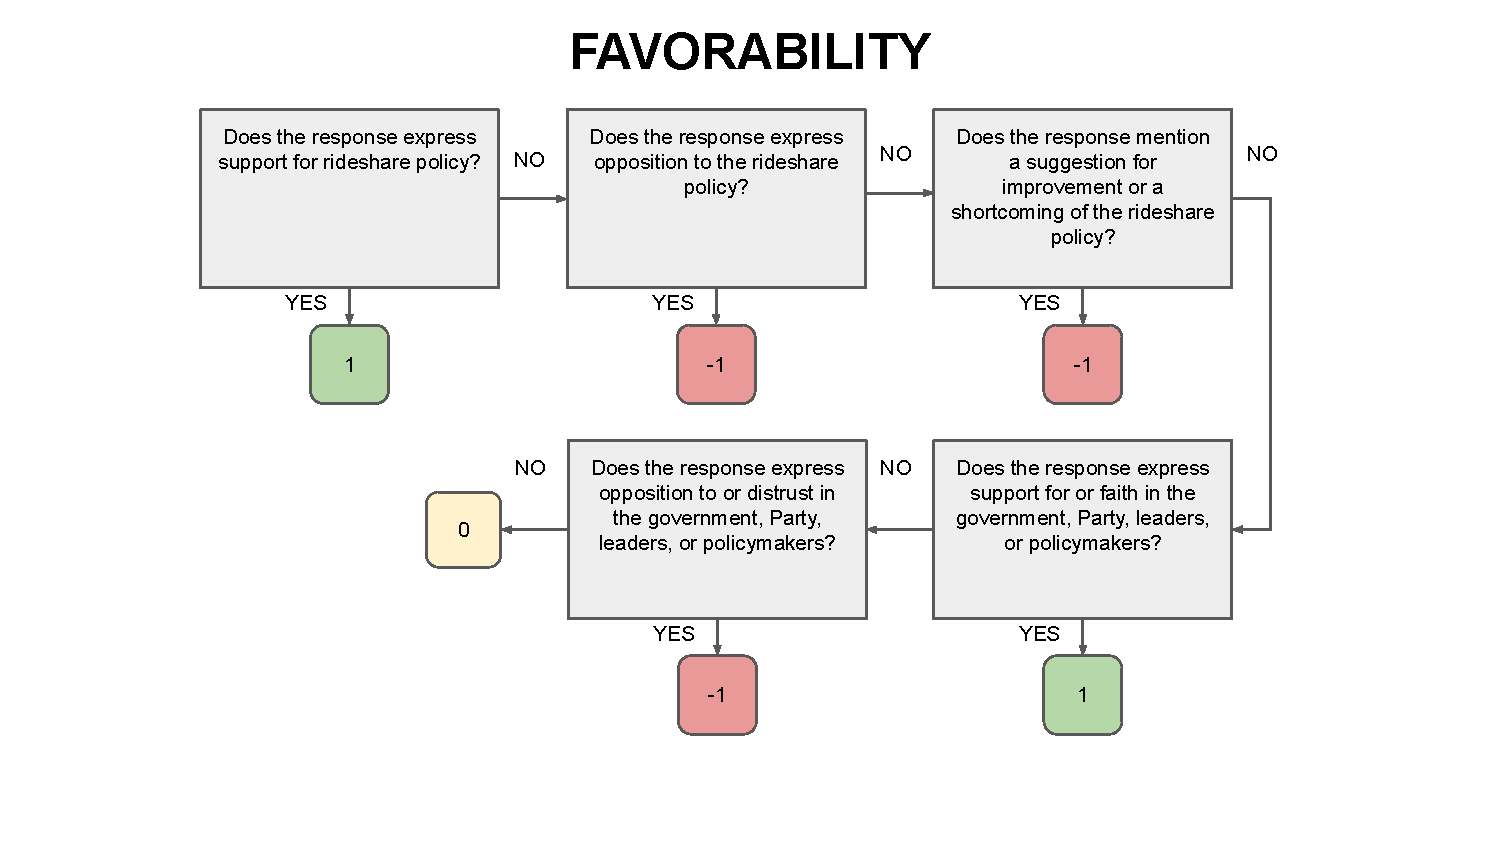
\includegraphics[width=\textwidth]{figures/coding_diagrams/favorability.pdf}
  \label{favorability}
\end{figure}

\begin{figure}
  \centering
  \caption{Nationalism Coding Diagram}
  \vspace{1em}
  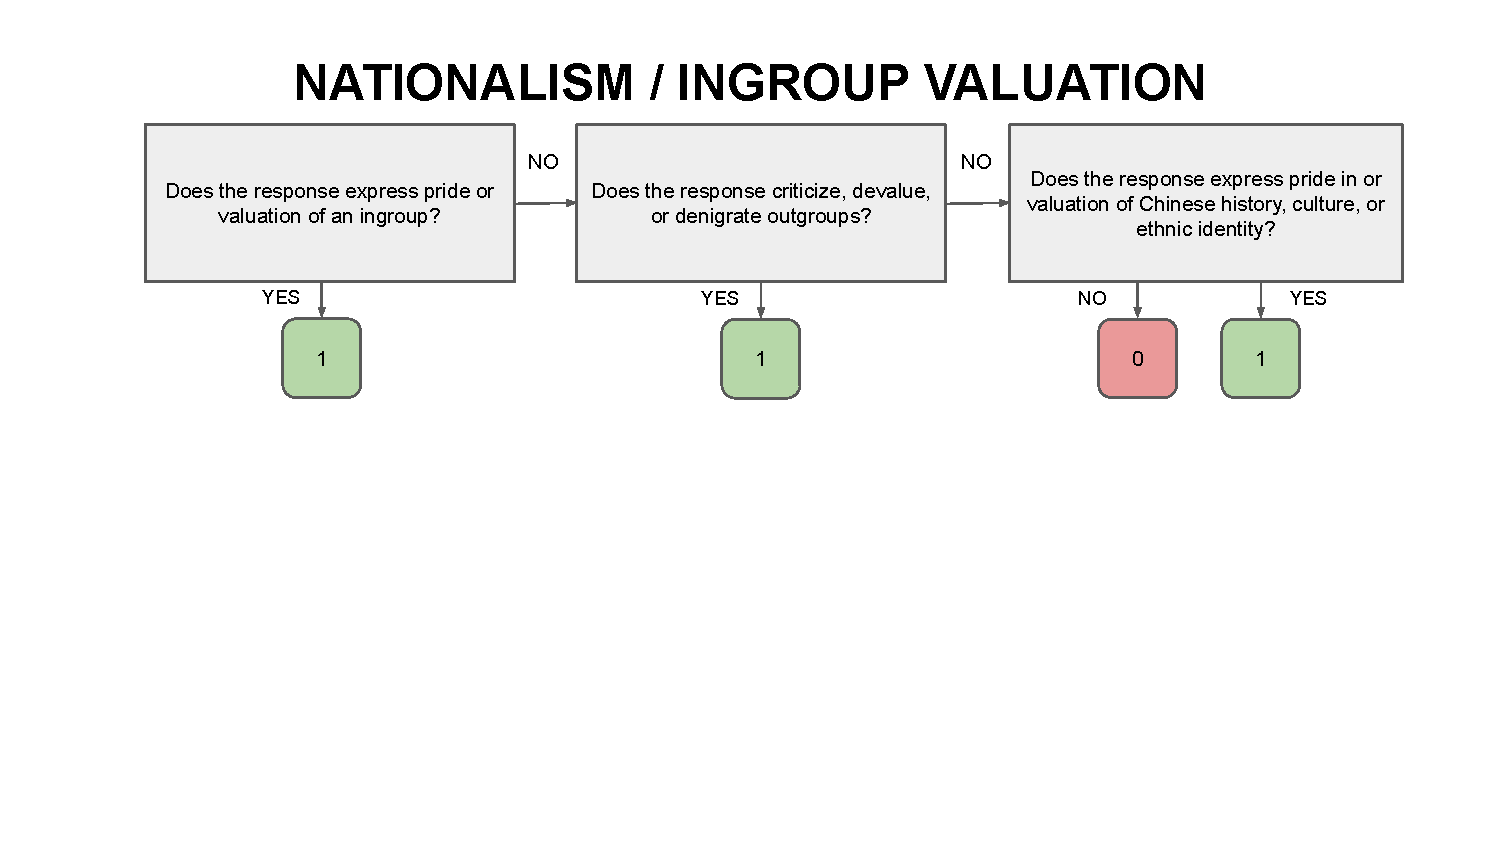
\includegraphics[width=\textwidth]{figures/coding_diagrams/nationalism.pdf}
  \label{nationalism}
\end{figure}

\begin{figure}
  \centering
  \caption{Discourse Competition Coding Diagram}
  \vspace{1em}
  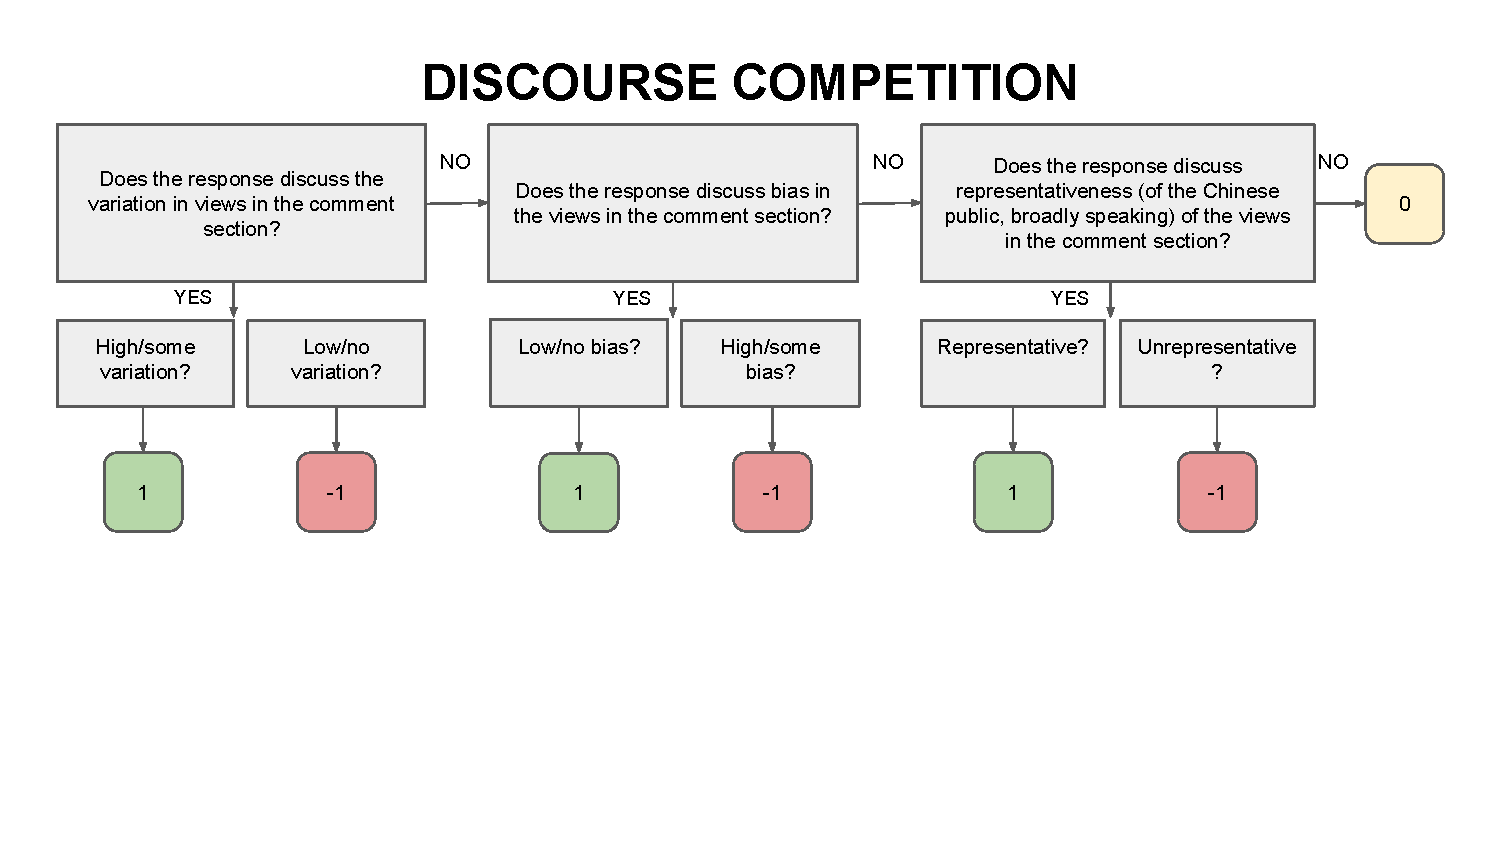
\includegraphics[width=\textwidth]{figures/coding_diagrams/discourse_competition.pdf}
  \label{discourse_competition}
\end{figure}

\newpage

\bibliographystyle{apacite}
\bibliography{info_control}

\end{document}